\chapter{ಜೀವವಿಜ್ಞಾನ}

(ತಾರೀಖು ೨೯.೧೨.೧೯೬೬ ರಿಂದ ತಾರೀಖು ೧೪.೦೧.೧೯೬೭ ವರೆಗೆ ಹೆಡೆತಲೆಯಲ್ಲಿ ದಿವ್ಯದಂಪತಿಗಳ ಸನ್ನಿಧಿಯಲ್ಲಿದ್ದ ಅನುಗ್ರಹಿಸಿದ ವಿಷಯ. ಸಂಗ್ರಹಿಸಿದವರು ಡಾ|| ಟ್. ಶ್ರೀನಿವಾಸ್)

\section*{ಭೌತಿಕಜೀವನದ ಹಿಂದೆ ದೈವಿಕ ಆಧ್ಯಾತ್ಮಿಕ ಕ್ಷೇತ್ರಗಳುಂಟು}

ನಾವು ಅನಂತಕಾಲದ ಪ್ರವಾಹದ ಮಧ್ಯೆ ಜೀವಿಗಳಾಗಿ ಹುಟ್ಟಿಬಂದು ಭೌತಿಕವಾದ ದೇಹವನ್ನು ಧರಿಸಿ ಜೀವನ ನಡೆಸುತ್ತಿದ್ದೇವೆ. ಇಂತಹ ಈ ಜೀವನದ ಬಗ್ಗೆ ತಿಳಿಯಬೇಕಾದ ಜವಾಬ್ದಾರಿಯಿದೆ ಈ ಬಗ್ಗೆ ಆಧುನಿಕವಿಜ್ಞಾನಿಯು ಹೊಂದಿರುವ ದೃಷ್ಟಿಕೋಣವು ಒಂದು ಸಂಕುಚಿತ ವ್ಯಾಪ್ತಿಯ ಸೀಮಿತ ಕ್ಷೇತ್ರವನ್ನು ಮಾತ್ರ ಒಳಗೊಂಡಿರುತ್ತದೆ. ನಿಸರ್ಗಸಹಜವಾಗಿ ವಸ್ತುಗಳ ವಿಕಾಸ ನಡೆಸುಕೊಂಡು ಬರುತ್ತಿದೆ. ಅದರಲ್ಲಿ ಹೊರಗಣ್ಣಿನಿಂದ ನೋಡಬಹುದಾದುದು ಭೌತಿಕವಾದುದು ಮಾತ್ರ. ಉಳಿದಿರುವ ಭಾಗ ದೈವಿಕ ಮತ್ತು ಆಧ್ಯಾತ್ಮಸಂಬಂಧವಾದುದು.

\section*{ಜೀವನದ ಬಗ್ಗೆ ಆಧುನಿಕವಿಜ್ಞಾನಿಗಳ ಹಾಗೂ ಋಷಿಗಳ ನೋಟ}

ಒಂದು ವಸ್ತುವನ್ನು ಅದರ ನಿಸರ್ಗದ ಪರಿಧಿಯಿಂದ ಹೊರತೆಗೆದು ನೋಡಿದಾಗ ಅದರ ನಿಸರ್ಗ ಸಹಜವಾದ ಹಿನ್ನೆಲೆಯನ್ನು ಬಿಟ್ಟು ಆಂಶಿಕವಾದ ರೀತಿಯಲ್ಲಿ ಅದರ ಅಭ್ಯಾಸ ನಡೆಸುವುದಾಗಿದೆ. ಉದಾಹರಣೆಗೆ ಒಂದು ಹೂವನ್ನೋ ಎಲೆಯನ್ನೋ ಒಂದು ಗಿಡದಿಂದ ಬೇರ್ಪಡಿಸಿ ಪರೀಕ್ಷೆಗೆ ಒಳಪಡಿಸಿದಾಗ, ಆ ಹೂವು ಅಥವಾ ಎಲೆಗೆ ಚೈತನ್ಯವನ್ನು ಕೊಟ್ಟು ಧರಿಸಿಟ್ಟುಕೊಂಡಿದ್ದ ಜೀವವನ್ನು ಬಿಟ್ಟು ಕೇವಲ ಭೌತಿಕವಾದ ಭಾಗವಷ್ಟನ್ನೇ ಪರಿಕ್ಷೆ ನಡೆಸಿದಂತಾಗುತ್ತದೆ. ಆಧುನಿಕವಿಜ್ಞಾನಿಯು ಕಣ್ಣಿಗೆ ಗೋಚರಿಸಿವ ಭೌತಿಕ ಪ್ರಕೃತಿಯ ಹಿಂದೆ ಇರುವ ಜೀವಶಕ್ತಿಯನ್ನು ಗುರುತಿಸಲಾರ. ಮಹರ್ಷಿಗಳು ಈ ಸ್ಥಾವರ ಜಂಗಮಾತ್ಮಕವಾದ ಪ್ರಕೃತಿಯನ್ನೂ ಮತ್ತು ಈ ಸಮಸ್ತಪ್ರಕೃತಿಯ ಹಿಂದೆ ಇದ್ದುಕೊಂಡು ಅದರ ವೈವಿಧ್ಯಪೂರ್ಣವಾದ ವಿಕಾಸಕ್ಕೆ ಕಾರಣವಾದ ಜೀವ ಮತ್ತು ಜೀವದ ಹಿಂದಿರುವ ದೇವ ಇವರನ್ನೂ ಅರಿತುಕೊಂಡರು ಪ್ರಕೃತಿಯಲ್ಲಿರುವ ವೈವಿಧ್ಯಕ್ಕೂ ವಿಕಾರಗಳಿಗೂ ಕೇವಲ ಪ್ರಕೃತಿಯೇ ಕಾರಣವೆಂದು ಆಧುನಿಕವಿಜ್ಞಾನಿ ತಿಳಿದುಕೊಂಡು ತನ್ನ ಕೆಲಸ ನಡೆಸುತ್ತಾನೆ. ಆದರೆ ಜೀವವು ತ್ರಿಗುಣಗಳ ವೈಪರೀತ್ಯದಿಂದ ಉಂಟಾಗುವ ಕರ್ಮದ ಅವಸ್ಥೆಗಳಿಗೆ ಒಳಪಟ್ಟು ಹೊಂದುವ ವಿಕಾಸ ಇಲ್ಲವೇ ವಿಕಾರಗಳೇ ಪ್ರಕೃತಿಯ ವೈವಿಧ್ಯಕ್ಕೆ ಕಾರಣವೆಂದು ಮಹರ್ಷಿಗಳು ಅರಿತಿದ್ದರು. ಪ್ರಕೃತಿಯ ವೈವಿಧ್ಯವನ್ನು ಅರಿಯಲು ತ್ರಿಗುಣಗಳ ವ್ಯಾಪಾರಕ್ಕೆ ಒಳಪಟ್ಟ ಜೀವದ ಅವಸ್ಥಾಭೇದಗಳನ್ನು ತಿಳಿಯಲೇ ಬೇಕಾಗುವುದು ಎಂಬುದು ಋಷಿಗಳ ಅಭಿಪ್ರಾಯ. ಆದ್ದರಿಂದ ನಿಜವಾದ ಸಂಶೋಧನೆಯು ಪ್ರಕೃತಿಯ ಭಾಗವಷ್ಟನ್ನೇ ಒಳಗೊಂಡಿದ್ದರೆ ಸಾಲದು. ಪ್ರಕೃತಿಯ ಹಿಂದಿನ ಜೀವಕ್ಕೆ ಸಂಬಂಧಪಟ್ಟ ವಿಜ್ಞಾನವನ್ನೂ ಸಂಶೋಧನೆಯ ಅಂಗವಾಗಿ ಮಾಡಿಕೊಳ್ಳಬೇಕು.

\section*{ಆಧುನಿಕವಿಜ್ಞಾನದ ಸಂಶೋಧನೆಯಲ್ಲಿರುವ ನ್ಯೂನತೆ}

ವಿಶ್ವದಲ್ಲಿ ನಾನಾ ರೀತಿಯ ಜೀವಕೋಟಿಗಳನ್ನು ನೋಡುತ್ತೇವೆ. ಇವುಗಳಲ್ಲಿ ಒಂದೊಂದರ ವಿಕಾಸ ಒಂದೊಂದು ರೀತಿ ನಡೆಸಿರುತ್ತದೆ. ಇವುಗಳ ಸಂಶೋಧನೆ ನಡೆದು ಬೇರೆ ಬೇರೆ ವಿಜ್ಞಾನದ ಶಾಖೆಗಳು ಹುಟ್ಟಿಕೊಳ್ಳುತ್ತವೆ. ನಾನು ಸಸ್ಯಶಾಸ್ತ್ರಜ್ಞ, ನಾನು ಭೌತಶಾಸ್ತ್ರಜ್ಞ ಎಂದು ಮುಂತಾಗಿ ಜನಗಳು ನಾನಾರೀತಿ ಆಡಿ ಕೊಳ್ಳಬಹುದು. ಆದರೆ ಈ ಎಲ್ಲಾ ವಿಕಾಸವೈವಿಧ್ಯದ ಹಿಂದೆ ಕೆಲಸಮಾಡುವುದು ಒಂದೇ ಶಕ್ತಿ, ಒಂದೇ ಚೈತನ್ಯ. ಕೇವಲ ಹೊರಗಣ್ಣಿನಿಂದ ನೋಡಿದಾಗ ವಸ್ತುಗಳಲ್ಲಿ ಸಾಂಕರ್ಯ, ವಿಕಾರಗಳಿಂದಾಗಿ ಕಾಲದೇಶಗಳ ಸುಳಿಯಲ್ಲಿ ಸಿಕ್ಕಿ ಪರಿವರ್ತನೆಯುಂಟಾಗುತ್ತಿರುವುದನ್ನು ನೋಡಬಹುದು. ಈ ನಿತ್ಯಪರಿವರ್ತನಶೀಲವಾದ ಪ್ರಕೃತಿಯಷ್ಟನ್ನೇ ಸಂಶೋಧನೆಯ ಅಂಗವಾಗಿ ತೆಗೆದುಕೊಂಡಾಗ ಹೊಸ ಹೊಸ ಸಿದ್ಧಾಂತಗಳು ಹುಟ್ಟಿಕೊಳ್ಳುತ್ತವೆ. ಅಲ್ಲದೆ ಇಂದು ಸರಿ ಎಂದು ಒಪ್ಪಿದ ಒಂದು ಸಿದ್ಧಾಂತವನ್ನು ನಾಳೆ ಬದಲಾಯಿಸಬೇಕಾಗುತ್ತದೆ, ಏಕೆಂದರೆ ಆ ಸಿದ್ಧಾಂತವು ಪರಿವರ್ತನಶೀಲವಾದ ಪ್ರಕೃತಿಯ ಏಕದೇಶವನ್ನು ಮಾತ್ರ ಒಳಗೊಂಡಿರುತ್ತದೆ. ಆಟಂ (ಅನ್ನು) ಕೊನೆಯದಾದ ಅವಿಭಾಜ್ಯವಸ್ತುವೆಂದರು. ಅನಂತರ ಅದನ್ನು ಇನ್ನೂ ಚಿಕ್ಕದಾಗಿ ಎಲೆಕ್ಟ್ರಾನ್ ಪ್ರೋಟಾನ್ ಮುಂತಾಗಿ ಒಡೆಯಲು ಸಾಧ್ಯವಾಯಿತು. ಅಲ್ಲಿಗೆ ಮೊದಲನೆಯ ಸಿದ್ಧಾಂತವು ಉರುಳಿಬಿತ್ತು. ಮುಂದೆ ಕೆಲವು ವರ್ಷಗಳಲ್ಲಿ ಅಥವಾ ಯುಗಗಳಲ್ಲಿ ಎಲೆಕ್ಟ್ರಾನ್ ಪ್ರೋಟಾನಿನ ಇಂದಿನ ರಚನೆಯ ಸಿದ್ಧಾಂಟವೇ ಉಳಿಯದೇ ಪರಿವರ್ತನೆ ಹೊಂದಿದಾಗ ಇಂದಿನ ಸಿದ್ಧಾಂತಗಳ ಪಾಡೇನು?

\section*{ಜ್ಞಾನವಿಜ್ಞಾನಸಂಪನ್ನನಾದ ಯೋಗಿಯು ಸೃಷ್ಟಿಯನ್ನು ಆಮೂಲಾಗ್ರವಾಗಿ ಅರಿಯುತ್ತಾನೆ}

ಅದೇ ಜಾಗದಲ್ಲಿ ಜ್ಞಾನಿಯಾದ ವಿಜ್ಞಾನಿಯೊಬ್ಬನು ಎಲ್ಲ ಜಡಚರವಸ್ತುಗಳ ಹಿಂದೆ ಇರುವ ಒಂದು ಸದ್ವಸ್ತುವನ್ನು (ಜೀವವನ್ನು) ಮೂಲತಃ ಅರಿತುಕೊಂಡಿರುವಲ್ಲಿ, ಆ ಜೀವವು ತ್ರಿಗುಣಗಳ ವ್ಯಾಪಾರಕ್ಕೆ ಒಳಪಟ್ಟು ನಾನಾ ರೀರಿಯ ವಿಕಾಸ ಅಥವಾ ವಿಕಾರಗಳನ್ನು ಹೊಂದಿ ಬೇರೆ ಬೇರೆ ರೂಪಗಳಲ್ಲಿ ಕಂಡುಬರುವುದನ್ನು ಅರಿಯಬಲ್ಲನು. ಒಂದು ಸಸ್ಯವಾಗಲೀ ಪ್ರಾಣಿಯಾಗಲೀ ಮನುಷ್ಯನಾಗಲೀ ಎದುರುಗಡೆ ಇದ್ದಾಗ, ಜ್ಞಾನವಿಜ್ಞಾನಸಂಪನ್ನನಾದವನು ಅಂದುಕೊಳ್ಳುತ್ತಾನೆ `ಓಹೋ ಈ ಜೀವ ಇಲ್ಲಿದೆಯೇ! ಜನ್ಮಜನ್ಮಾಂತರದ ಕರ್ಮಗಳ ಸುಳಿಗೆ ಸಿಕ್ಕಿ  ತ್ರಿಗುಣಗಳ ವ್ಯಾಪಾರಕ್ಕೆ ಒಳಪಟ್ಟು ಈ ಜೀವ ಈ ಪಾಡು ಪಡುತ್ತಿದೆಯೇ? ಎಂದು. ಅಲ್ಲಿಗೆ ಅದು ಸಸ್ಯವಾಗಲೀ ಪ್ರಾಣಿಯಾಗಲೀ ಮನುಷ್ಯನಾಗಲೀ ಯಾವ ವಿಕಾಸ ಇಲ್ಲವೇ ವಿಕಾರದ ಅವಸ್ಥೆಯಲ್ಲಿರುವುದೋ ಅದೆಲ್ಲದರ ಹಿಂದಿನ ಗುಟ್ಟನ್ನು ಜ್ಞಾನಿಯು ಪತ್ತೆಹಚ್ಚಿ ಬಿಡುತ್ತಾನೆ. ಇಂತಹ ಜ್ಞಾನವಿಜ್ಞಾನಸಂನ್ನನು ಪ್ರಕೃತಿಯ ವೈವಿಧ್ಯವನ್ನೂ, ಅದ್ಭುತವನ್ನೂ ಕಂಡು ವಿಸ್ಮಯಗೊಳ್ಳುವುದಿಲ್ಲ.

\begin{shloka}
ಜ್ಞಾನವಿಜ್ಞಾನತೃಪ್ತ್ತಾತ್ಮಾ ಕೂಟಸ್ಥೋ ವಿಜಿತೇಂದ್ರಿಯಃ|\\
ಯುಕ್ತ ಇತ್ಯುಚ್ಯತೇ ಯೋಗೀ ಸಮಲೋಷ್ಟಾಶ್ಮಕಾಂಚನಃ||
\end{shloka}

(ಜ್ಞಾನ ಮತ್ತು ವಿಜ್ಞಾನ ಇವುಗಳಿಂದ ತೃಪ್ತಿ ಹೊಂದಿದ ಮನಸ್ಸುಳ್ಳವನೂ, ಕೂಟಸ್ಥನೂ (ದ್ವಂದ್ವಗಳಿಂಡ ವಿಕಾರ ಹೊಂದದೆ ಅಲುಗಾಡದವನು) ಜಿತೇಂದ್ರಿಯನೂ, ಮಣ್ಣು, ಕಲ್ಲು, ಚಿನ್ನ ಇವುಗಳನ್ನು ಸಮವಾಗಿ ನೋಡುವವನೂ ಆದ ಯೋಗಿಯೊಬ್ಬನು ಯುಕ್ತನೆಂದು ಹೇಳಲ್ಪಡುತ್ತಾನೆ) ಅಂತಹ ಯೋಗಿಯಾದವನು ಸೃಷ್ಟಿಯನ್ನು ಅರ್ಥಮಾಡಿಕೊಂಡವನಾಗಿದ್ದು ಅದನ್ನು ನೋಡಿ ಬೆಚ್ಚಿ ಬೀಳುವುದಿಲ್ಲ.

\section*{ಆಧುನಿಕವಿಜ್ಞಾನಿ ಹಾಗೂ ಜ್ಞಾನಿಯ ನೋಟದಲ್ಲಿರುವ ಅಂತರ}

ಬೀಜದಲ್ಲಿ ವೃಕ್ಷದ ಎಲ್ಲಾ ಲಕ್ಷಣಗಳೂ ಗುಪ್ತವಾಗಿ ಸೂಕ್ಷ್ಮವಾಗಿ ಅಡಗಿರುತ್ತವೆ. ಒಂದು ಜಾತಿಯ ಗಿಡದ ಎಲೆಯಲ್ಲಿ ಹತ್ತು ಚುಕ್ಕಿಗಳು ಬಿಡುವ ಗುಣವಿದ್ದರೆ, ಬೀಜದಲ್ಲಿ ಆ ಲಕ್ಷಣವನ್ನು ಉಂಟುಮಾಡುವ ಸೂಕ್ಷ್ಮಾಂಶಗಳು ಇರಲೇಬೇಕಷ್ಟೆ. ಈ ಎಲ್ಲಾ ಲಕ್ಷಣಗಳನ್ನೂ ಇಟ್ಟುಕೊಂಡು ಬೀಜವು ತನ್ನ ನಿಸರ್ಗ ಸಹಜವಾದ ದಾRಇಯಲ್ಲಿ ವಿಕಾಸ ಹೊಂದಲು ಪ್ರಾರಂಭಿಸಿದಾಗ ಬೀಜದಿಂದ ಅಂಕುರ, ಕಾಂಡ, ಎಲೆ, ಹೂ, ಕಾಯಿ ಎಲ್ಲವೂ ಆಗಿ ಮತ್ತೆ ಬೀಜದಲ್ಲಿ ನಿಲ್ಲುತ್ತದೆ. ಕೇವಲ ಒಂದು ಎಲೆಯನ್ನೋ, ಹೂವನ್ನೋ, ಕಾಯಿಯನ್ನೋ ಸಂಶೋಧನೆಯ ವಿಷಯವಾಗಿ ತೆಗೆದುಕೊಂಡಾಗ, ಬೀಜದಿಂದ ವೃಕ್ಷ ಬೆಳೆದು ಮತ್ತೆ ಬೀಜದಲ್ಲಿ ನಿಲ್ಲುವ ಸಕಲವ್ಯಾಪಾರಗಳ ಏಕಸೂತ್ರತೆಯ ಸಮಗ್ರವಾದ ಅರಿವುಂಟಾಗಲು ಸಾಧ್ಯವಿಲ್ಲವಷ್ಟೆ. ಆದ್ದರಿಂದ ಆಧುನಿಕವಿಜ್ಞಾನಿಯು ನೋಡುವುದು ಒಂದೊಂದು ಅಂಶವನ್ನು, ಜ್ಞಾನಿ ನೋಡುವುದು (ಎಲ್ಲಾ ಅಂಶಗಳುಳ್ಳ) ಅಂಶಿಯನ್ನು.

\section*{ಸೃಷ್ಟಿಯಲ್ಲಿ ವಿಕಾರವೇರ್ಪಟ್ಟರೆ ಮೂಲ ತಲುಪಲಾಗುವುದಿಲ್ಲ}

ಸೃಷ್ಟಿಯಲ್ಲಿ ಒಂದು ನಿಯಮವುಂಟು, ಆದರ ಒಂದು ಆಶಯವುಂಟು, ಅದರ ವಿಕಾಸಕ್ಕೆ ಒಂದು ಕ್ರಮವುಂಟು, ಈ ಕ್ರಮವಾದ ವಿಕಾಸವು ವ್ಯತ್ಯಾಸವವಾದಾಗ ಸೃಷ್ಟಿಯಲ್ಲಿ ವಿಕಾರ. ಒಂದು ಕೇಂದ್ರವಿಟ್ಟುಕೊಂಡು ಒಂದು ವೃತ್ತವನ್ನು ಬೆಳೆಸಲು ಹೊರಟಾಗ ಅದರ ಮುನ್ನಡೆಯು ಕ್ರಮವಾಗಿದ್ದರೆ ಆ ರೇಖೆಯು ಬಳಸಿಬಂದು ಪುನಃ ಆ ಮೂಲವನ್ನೇ ತಲುಪಿ ಒಂದು ಪೂರ್ಣ ವೃತ್ತವಾಗುತ್ತದೆ. ಒಂದು ಬೇಳೆ ಅಡ್ಡದಾರಿ ಹಿಡಿದು ರೇಖೆ ಮುಂದುವರಿದರೆ ತನ್ನ ಮೂಲಕ್ಕೆ ಬಂದು ತಲುಪುವ ಬದಲು ಸುಮ್ಮನೆ ಸುತ್ತುತ್ತಿರುತ್ತದೆ.

ಉದಾಹರಣೆ:-
\begin{center}
\includegraphics{chap5-fig1.eps}
\end{center}

\section*{ಸೃಷ್ಟಿಯ ವೈವಿಧ್ಯದ ಹಿಂದೆ ಒಂದೇ ಮೂಲವಿದೆ}

ಸೃಷ್ಟಿ ಎಷ್ಟೇ ವೈವಿಧ್ಯಪೂರ್ಣವಾಗಿ ಹೊರಗಡೆ ಕಂಡುಬಂದರೂ ಅದರ ಮೂಲದಲ್ಲಿ ಏಕತೆಯೂ, ಸಮಾನತೆಯೂ, ಸಮರಸತೆಯೂ ಉಂಟು ಸೃಷ್ಟಿಯು ವಿಕಾಸದ ಹಾದಿ ಹಿಡಿದು ಹೊರಟಾಗ ವೈವಿಧ್ಯಪೂರ್ಣವಾದ ರೂಪ, ಆಕಾರಗಳನ್ನು ಹೊಂದಿದರೂ ತನ್ನ ಮೂಲಸ್ವರೂಪವನ್ನು ಕೆಡಿಸಿಕೊಳ್ಳದೆ ತನ್ನೊಡನೆಯೇ ಹೊತ್ತು ಕೊಂಡು ಬಂದು ಮತ್ತೆ ಕೊನೆಯಲ್ಲಿ ತನ್ನ ಮೂಲ ಸ್ವರೂಪದಲ್ಲಿಯೇ ನಿಲ್ಲುತ್ತದೆ. ಜ್ಞಾನವಿಜ್ಞಾನಸಂಪನ್ನನಾದವನು ಸೃಷ್ಟಿಯ ಈ ಮೂಲಸ್ವರೂಪದಲ್ಲಿಯೇ ನಿಲ್ಲುತ್ತದೆ. ಜ್ಞಾನವಿಜ್ಞಾನಸಂಪನ್ನನಾದವನು ಸೃಷ್ಟಿಯ ಈ ಮೂಲಸ್ವಾರೂಪವನ್ನೂ ಮತ್ತು ಸೃಷ್ಟಿಯ ಆಶಯವನ್ನೂ ಚೆನ್ನಾಗಿ ಅರಿತಿರುತ್ತಾನೆ.

\begin{shloka}
ವಿದ್ಯಾವಿನಯಸಂಪನ್ನೇ ಬ್ರಾಹ್ಮಣೇ ಗವಿ ಹಸ್ತಿನಿ |\\
ಶುನಿ ಚೈವ ಶ್ವಪಾಕೇ ಚ ಪಂಡಿತಾಸ್ಸಮದರ್ಶಿನಃ ||
\end{shloka}

(ಅಂತಹ ಜ್ಞಾನಿಗಳು ವಿದ್ಯಾವಿನಯಸಂಪನ್ನನಾದ ಬ್ರಾಹ್ಮಣನಲ್ಲಿಯೂ, ಗೋವಿನಲ್ಲಿಯೂ, ಆನೆಯಲ್ಲಿಯೂ, ನಾಯಿಯಲ್ಲಿಯೂ ಮತ್ತು ನಾಯಿಯನ್ನು ತಿಂದು ಜೀವಿಸುವ ಮನುಷ್ಯನಲ್ಲಿಯೂ ಇರುವ ರೂಪ, ಆಕಾರ, ಗುಣಭೇದಗಳನ್ನು ಹೊರಗಣ್ಣಿನಿಂದ ನೋಡುತ್ತಿದ್ದರೂ ಅವೆಲ್ಲವುಗಳ ಮೂಲದಲ್ಲಿ ಇರುವ ಅಂದರೆ ಜೀವಸ್ಥಾನದಲ್ಲಿರುವ ಸಮಾನತೆಯನ್ನು ಒಳಗಣ್ಣಿನಿಂಡ ನೋಡುತ್ತಾರೆ.) ಎಲ್ಲಾ ರೀತಿಯ ವೈವಿಧ್ಯಗಳೂ ಒಂದೇ ಮೂಲದ ಬೇರೆ ಬೇರೆ ರೀತಿಯ ವಿಕಾಸ ಕ್ರಮಗಳಾಗಿವೆ.

\section*{ಸೃಷ್ಟಿಯ ವೈವಿಧ್ಯದ ಕಾರಣಗಳು}

ಮೂಲದಲ್ಲಿ ಸಮಾನವಾಗಿರುವ ಜೀವವು ತ್ರಿಗುಣಗಳ ವ್ಯಾಪಾರಕ್ಕೆ ಒಳಪಟ್ಟು ಕರ್ಮಫಲವನ್ನು ಭೋಗಿಸುವ ಸಲುವಾಗಿ ಜನ್ಮತಾಳಿದೆ. ಇಂದು ಪ್ರಾಣಿಯಾಗಿ ಜನ್ಮವೆತ್ತಿದ ಜೀವವು ಮುಂದೆ ಮನುಷ್ಯನಾಗಿ ಜನ್ಮವೆತ್ತಬಹುದು. ಹೀಗೆ ಒಂದೇ ಜೀವವು ನಾನಾರೀತಿಯ ಜನ್ಮವನ್ನು ತಾಳಬಹುದು. ಇದರಿಂದ ತಿಳಿಯಬೇಕಾದುದೇನೆಂದರೆ ಜೀವವು ಮೂಲದಲ್ಲಿ ಸಮಾನವಾಗಿದೆ. ಹೊರಗಡೆ ಕಂಡುಬರುವ ವೈವಿಧ್ಯಗಳು, ಕರ್ಮಗಳ ಮತ್ತು ಗುಣಗಳ್ ವ್ಯಾಪಾರದಿಂದ ಉಂಟಾಗಿವೆ. ಪ್ರಕೃತಿಯನ್ನೂ ಮತ್ತು ಜೀವವನ್ನೂ ಬೇರೆ ಬೇರೆಯಾಗಿಯೂ ಸಮಗ್ರವಾಗಿಯೂ ಅರಿಯಬಲ್ಲ ವಿಜ್ಞಾನಿಗೆ, ಯಾವ ಸೃಷ್ಟಿ ಏಕಾಯಿತು? ಹೇಗಾಯಿತು? ಇದು ಸೃಷ್ಟಿಯ ಆಶಯಕ್ಕೆ ಹೊಂದಿಕೊಂಡು ಕ್ರಮವಾದ ವಿಕಾಸದ ಹಾದಿಯಲ್ಲಿ ನಡೆದಿದೆಯೇ? ಅಥವಾ ಅಕ್ರಮವಾದ ಮುನ್ನಡೆಯಿಂದ ವಿಕಾರವಾದ ರೂಪ ತಾಳಿದೆಯೇ? ಎಂಬೆಲ್ಲ ವಿಷಯಗಳೂ ಸುಬೋಧವಾಗುತ್ತವೆ.

\section*{ಭೌತಿಕಸೃಷ್ಟಿಯನ್ನೇ ಅವಲೋಕಿಸಿದರೂ ಒಂದು ಮೌಲಿಕವಾದ ಸಮಾನತೆಯಿದೆ}

ಆಧುನಿಕ ವಿಜ್ಞಾನಿಯ ದಾರಿಯಲ್ಲಿಯೇ ಹೊರಟು ಕೇವಲ ಭೌತಿಕವಾದ ಸೃಷ್ಟಿಯನ್ನೇ ಅವಲೋಕಿಸಿ ನೋಡಿದಾಗಲೂ, ಸೃಷ್ಟಿಯ ವಿಕಾಸ ಅಥವಾ ವಿಕಾರಗಳಿಂದ ಉಂಟಾದ ವೈವಿಧ್ಯಗಳ ಹಿಂದೆ ಇರುವ ಸಮಾನತೆಯನ್ನು ಕಂಡುಕೊಳ್ಳಬಹುದಾಗಿದೆ. ಉದಾಹರಣೆಗೆ- ನಾನಾ ರೀತಿಯ ಪ್ರಾಣಿಗಳ ಮತ್ತು ಮನುಷ್ಯರ ಭ್ರೂಣದಶೆಯಿಂದ ಹಿಡಿದು ಮುಂದಿನ ಶರೀರದ ಬೆಳವಣಿಗೆಯ ವಿಕಾಸಕ್ರಮವನ್ನು ತೋರಿಸುವ ಚಿತ್ರಗಳನ್ನು ಸಾಲಾಗಿ ಇಟ್ಟರೆ, ಇದರಿಂದ ಕಂಡುಬರುವುದೇನೆಂದರೆ, ಎಲ್ಲಾ ಪ್ರಾಣಿಗಳ ಶರೀರ ರಚನೆಯೂ ಭ್ರೂಣದಶೆಯ ಪ್ರಾರಂಭದಲ್ಲಿ ಒಂದೇ ಪ್ರಕಾರವಾಗಿದೆ.

\begin{center}

\includegraphics{chap5-fig2.eps}
\end{center}

ಇದ್ದು ಬರಬರುತ್ತಾ ಬೇರೆ ಬೇರೆ ರೂಪವನ್ನು ತಾಳುತ್ತವೆ. ಜೀವಮೂಲದ ಸಮಾನತೆಯನ್ನು ಇದರಿಂದ ತಿಳಿದುಕೊಳ್ಳಬಹುದಾಗಿದೆ.

\section*{ಜೀವಮೂಲದ ಏಕರೂಪತೆಗೆ ಗೀತೆಯ ಪ್ರಮಾಣವಚನ}

ಈ ಜೀವಮೂಲದ ಸಮಾನತೆಗೆ ಆಧಾರವೇನೆಂದರೆ, ಸನಾತನವಾದ ಈ ಎಲ್ಲಾ ಜೀವವಿಶೇಷಗಳೂ ಪರಮಾತ್ಮನ ಅಂಶಗಳಾಗಿರುವುದೇ ಆಗಿದೆ. ಬೇರೆ ಬೇರೆ ಜೀವವ್ಯಾಪಾರಗಳ ಹಿಂದೆ ತನ್ನ ಶಕ್ತಿಯ ಅಂಶದ ವಿಸ್ತಾರವೇ ಕೆಲಸ ಮಾಡುತ್ತಿರುವುದನ್ನು ಭಗವಂತನು ಗೀತೆಯ ಹತ್ತನೇ ಅಧ್ಯಾಯದಲ್ಲಿ ವಿಸ್ತಾರವಾಗಿ ತಿಳಿಸಿರುತ್ತಾನೆ. `ನಾನು ನಕ್ಷತ್ರಗಳಲ್ಲಿ ಚಂದ್ರನಾಗಿದ್ದೇನೆ. ದೇವತೆಗಳಲ್ಲಿ ಇಂದ್ರನಾಗಿದ್ದೇನೆ, ಮಹರ್ಷಿಗಳಲ್ಲಿ ಭೃಗುವಾಗಿದ್ದೇನೆ, ಉತ್ತಮ ಗಜಗಳಲ್ಲಿ ಐರಾವತವಾಗಿದ್ದೇನೆ, ಮನುಷ್ಯರಲ್ಲಿ ರಾಜನೆಂದು ನನ್ನನ್ನು ತಿಳಿದುಕೋ' ಮುಂತಾಗಿ ಸೃಷ್ಟಿಯಲ್ಲಿ ತನ್ನ ವಿಶ್ವವ್ಯಾಪಕವಾದ ಮತ್ತು ಏಕಮೂಲವಾದ ಅಸ್ತಿತ್ವವನ್ನು  ಸ್ಪಷ್ಟಪಡಿಸಿದ್ದಾನೆ.

\section*{ಸೃಷ್ಟಿಯ ವಿಕಾಸದಲ್ಲಿ ಮೂಲಕ್ಕೆ ಸೇರುವ ನಡೆಯಿದೆ}

ಈ ರೀತಿಯಲ್ಲಿ ಸತ್ಯವನ್ನೇ ಮೂಲವಾಗಿ ಉಳ್ಳ ಸೃಷ್ಟಿಯ ವಿಕಾಸಕ್ಕೆ ಅರ್ಥವೇನು? ಆಶಯವೇನು? ಎಂಬುದನ್ನು ಜ್ಞಾನವಿಜ್ಞಾನಸಂಪನ್ನನ್ನು ಮಾತ್ರ ಅರಿಯಬಲ್ಲನು. ಸೃಷ್ಟಿಯು ತನ್ನ ಸತ್ಯದ ಸ್ಥಾನದಿಂದ ವಿಕಾಸದ ಮೆಟ್ಟಲನ್ನು ಏರಿ, ಸೃಷ್ಟಿ ಸ್ಥಿತಿ ಲಯಗಳ ರೂಪದಲ್ಲಿ ಒಂದು ನಿಯಮಿತವಾದ, ಕ್ರಮಬದ್ಧವಾದ ಅಕ್ಷದಲ್ಲಿ ತನ್ನ ಗತಿಯನ್ನು ಹೊಂದಿದೆ. ತನ್ನ ಮೂಲ ಸ್ವರೂಪವನ್ನೂ ಆಶಯವನ್ನೂ ಸೃಷ್ಟಿಯು ತನ್ನ ವಿಕಾಸದ ಉದ್ದಕ್ಕೂ ಕಾಯ್ದಿಟ್ಟುಕೊಂಡು ಪುನಃ ತನ್ನ ಸ್ವಸ್ವರೂಪದಲ್ಲೇ ನಿಲ್ಲುತ್ತದೆ. ಇದೇ ಸೃಷ್ಟಿಯ ಸ್ವಾಭಾವಿಕ ವಿಕಾಸದ ಗತಿಯೂ ಮತ್ತು ಆಶಯವೂ ಆಗಿದೆ.

ಉದಾಹರಣೆಗೆ ೯ರ ಮಗ್ಗಿಯನ್ನು ತೆಗೆದುಕೊಳ್ಳೋಣ. ಇಲ್ಲಿ ೯ ಎಂಬ ವಿಶೆಷ್ಯವು ೧ ಎಂಬ ವಿಶೇಷಣದೊಂದಿಗೆ ಸೇರಿ ೯ ಆಗಿ ಉಳಿಯುತ್ತದೆ. ಇದೇ ರೀತಿ ೯$\times$೨ ರಲ್ಲಿ ೯ ಎಂಬ ವಿಶೇಷ್ಯವು ೨ ಎಂಬ ವಿಶೇಷ್ಯವು ವಿಶೇಷಣದೊಂದಿಗೆ ಕೂಡಿ, ತನ್ನ ವಿಸ್ತಾರವನ್ನು ಮಾಡಿಕೊಂಡು ೧೮ ಆಯಿತು. ಆದರೆ ೧$+$೮ = ೯ ಎಂಬ ಅರ್ಥದಲ್ಲಿ ತನ್ನ ಮೂಲ ರೂಪವಾದ ೯ನ್ನು ಕಾಯ್ದಿಟ್ಟು ಕೊಂಡಿದೆ. ಮುಂದೆ ೯ ಎಂಬ ಅರ್ಥದಲ್ಲಿ ತನ್ನ ಮೂಲ ರೂಪವಾದ ೯ನ್ನು ಕಾಯ್ದಿಟ್ಟು ಕೊಂಡಿದೆ. ಮುಂದೆ ೯ ಎಂಬ ವಿಶೇಷ್ಯವು ೩ ರಿಂದ ಹಿಡಿದು ೧೦ರ ವರೆಗಿನ ವಿಶೇಷಣದೊಂದಿಗೆ ಸೇರಿ ವಿಸ್ತಾರಗೊಂಡರೂ, ಆ ವಿಸ್ತಾರಗೊಂಡ ಸಂಖ್ಯೆಗಳನ್ನು ಕೂಡಿ ನೋಡಿದಾಗ ೯ ಎಂಬ ಸಂಖ್ತ್ಯೆಯೇ ಬರುತ್ತದೆ. ಕೊನೆಯಲ್ಲಿ ೯$\times$೧೦ = ೯೦ ಆಗಿ ತನ್ನ ಮೂಲರೂಪದಲ್ಲಿ ಬಂದು ನಿಲ್ಲುತ್ತದೆ. ಇದೇ ರೀತಿ ೧೮, ೩೯ ಮುಂತಾದ ೯ರ ವಿಸ್ತಾರರೂಪವಾದ ಸಂಖ್ಯ್ತೆಗಳ ಮಗ್ಗಿಯಲ್ಲಿಯೂ ವಿಕಾಸದ ಕ್ರಮಬದ್ಧರೀತಿಯನ್ನು ನೋಡಬಹುದು.

ಹೀಗೆಯೇ ಸಂಖ್ಯೆಯ ಬೆಳವಣಿಗೆಯೂ ಸಹ ತನ್ನ ಮೂಲರೂಪವನ್ನು ಉದ್ದಕ್ಕೂ ಕಾಯ್ದಿಟ್ಟುಕೊಳ್ಳುತ್ತದೆ. ಉದಾಹರಣೆಗೆ ೧ ಎಂಬ ಮೂಲ ಸಂಖ್ಯೆಯು ಮತ್ತೆ ೧ರ ಜೊತೆ ಸೇರಿ ೨ ಆಯಿತು. ಇಲ್ಲಿ ೨, ೧ರ ವಿಕಾಸ ರೂಪವಾಗಿದೆ. ಈ ರೀತಿ ೩, ೪ ಇತ್ಯಾದಿ ಸಂಖ್ಯೆಗಳಲ್ಲಿ ಅದು ತನ್ನ ಬೃದ್ಧಿಯನ್ನು ತೋರ್ಪಡಿಸಿಕೊಂಡು ಕೊನೆಯಲ್ಲಿ ೧೦ರಲ್ಲಿ ಬಂದು ನಿಲ್ಲುತ್ತದೆ. ತನ್ನ ಬೆಳವಣಿಗೆಯ ಉದ್ದಕ್ಕೂ ೧ ಎಂಬ ಮೂಲರೂಪವನ್ನು ಕಾಯ್ದಿಟ್ಟುಕೊಂಡು ಬಂದು ಕೊನೆಯಲ್ಲಿ ೧೦ ಎಂಬ ಸಂಖ್ಯೆಯಲ್ಲಿ ತನ್ನ ಆ ರೂಪವನ್ನು  ಹೊರಗೆಡಹುತ್ತದೆ. ಇದು ಸೃಷ್ಟಿಯ ಸ್ವಾಭಾವಿಕವಾದ ವಿಕಾಸದ ರೀತಿಯಾಗಿದೆ.

\section*{ಜ್ಞಾನವಿಜ್ಞಾನಗಳೆಂದರೇನು?}

ಜ್ಞಾನಿಯಾದವನು ಕಾರ್ಯಕಾರನ ಸಂಬಂಧವನ್ನು ಅರಿತು ಸೃಷ್ಟಿಯ ಈ ವಿಕಾಸ ಕ್ರಮವನ್ನು ತಿಳಿದುಕೊಂಡಾಗ ವಿಜ್ಞಾನಿ ಎನ್ನಿಸಿಕೊಳ್ಳುತ್ತಾನೆ. ವಿಶೇಷ್ಯ ವಿಶೇಷಣಗಳು ಕೂಡಿ ಉಂಟಾಗುವುದು ವಿಕಾಸ. ಈ ವಿಕಾಸದ ಸಮಗ್ರತೆಯನ್ನು ಅರಿತುಕೊಳ್ಳುವುದು ವಿಜ್ಞಾನ. ಕೇವಲ ವಿಶೇಷ್ಯವನ್ನು ಅರಿಯುವುದು ಜ್ಞಾನ. ಬೀಜದ ಸ್ಥಿತಿಯಲ್ಲಿ ನಿಂತಾಗ ಜ್ಞಾನ. ವೃಕ್ಷ ಬೀಜಗಳ ಸಮಗ್ರತೆಯನ್ನು ಏಕನೋಟದಿಂದ ನೋಡುವುದು ವಿಜ್ಞಾನ.

\section*{ಲೋಕದಲ್ಲಿ ವಿಜ್ಞಾನಿಯ ಕರ್ತವ್ಯ}

ಇಂಟಹ ಜ್ಞಾನವಿಜ್ಞಾನಸಂಪನ್ನನಾದ ವಿಜ್ಞಾನಿಯು ಲೋಕದಲ್ಲಿ ಮಾಡ ಬೇಕಾದುದು ಅಥವಾ ಮಾಡಬಯಸುವುದು ಏನು? ಎಂದರೆ ಸೃಷ್ಟಿಯನ್ನು ಅದರ ಆಶಯದೊಂದಿಗೆ ಅರ್ಥಮಾಡಿಕೊಂಡು, ಅದರ ಸ್ವಾಭಾವಿಕ ವಿಕಾಸಕ್ಕೆ ಅಡೆತಡೆಯುಂಟಾಗಿದ್ದರೆ, ಆ ಗಂಟನ್ನು ಬಿಡಿಸಿ ಅದರ ಮುನ್ನಡೆಗೆ ಅವಕಾಶ ಮಾಡಿಕೊಡುವುದೇ ಆಗಿದೆ. ಸೃಷ್ಟಿಯಲ್ಲಿ ಅಡಕವಾಗಿರುವ ವಿಶಯ ಅಥವಾ ವಸ್ತುಗಳನ್ನು ತನ್ನ ಕೈಗೆ ತೆಗೆದುಕೊಂಡು ಅದಕ್ಕೆ ಸೃಷ್ಟಿಗೆ ಸಹಜವಲ್ಲದ ಬೇರೆ ವಿಧವಾದ ರೂಪವನ್ನು ಕೊಡಲು ಪ್ರಯತ್ನಿಸುವುದು ನಿಜವಾದ ವಿಜ್ಞಾನಿಯ ಕರ್ತವ್ಯವಲ್ಲ.

\section*{ಆಧುನಿಕವಿಜ್ಞಾನವು ಹೇಗೆ ಬೆಳೆದರೆ ಚೆನ್ನು}

ಆದರೆ ಆಧುನಿಕ ವಿಜ್ಞಾನಿಯು ತನ್ನ ಬುದ್ಧಿ ಶಕ್ತಿಯ ಆಧಾರದ ಮೇಲೆ ಇಂತಹ ಸೃಷ್ಟಿಗೆ ಸಹಜವಲ್ಲದ ಹೊಸ ಹೊಸ ಸಂಶೋಧನೆಗಳನ್ನೂ ಬದಲಾವಣೆಗಳನ್ನೂ ಮಾಡಲು ಹೊರಟಿದ್ದಾನೆ. ಸೃಷ್ಟಿಯು ಯಾವುದೋ ಒಂದು ನಿಯಮಕ್ಕೆ ಒಳಪಟ್ಟು ಪರಸ್ಪರ ಹೊಂದಾಣಿಕೆಯಿಂದ ವಿಕಾಸಶೀಲವಾಗಿ ಮುಂದುವರಿಯುತ್ತಿದೆ. ಈ ಪರಸ್ಪರ ಸಂಬಂಧವನ್ನೂ, ಹೊಂದಾಣಿಕೆಯನ್ನೂ ಸಮಗ್ರವಾಗಿ ಅರಿತುಕೊಳ್ಳದೆ ಏಕದೇಶೀಯವಾದ ನೋಟದಿಂದ ಸಂಶೋಧನೆಯನ್ನು ನಡೆಸುವುದಾಗಲೀ ಬದಲಾವಣೆಗಳನ್ನು ಕೃತಕವಾಗಿ ಉಂಟುಮಾಡುವುದಾಗಲೀ ಸೃಷ್ಟಿಯ ನಿಯಮಬದ್ಧವಾದ ಸ್ಥಿತಿಗೆ ಹಾನಿಕರ.

ಕೃತಕವಾದ ಒಂದು ಬದಲಾವಣೆಯಿಂದ, ಬಾಹ್ಯನೋಟಕ್ಕೆ ಒಂದು ಸಮಸ್ಯೆಯು ಪರಿಹಾರವಾದಂತೆ ತೋರಬಹುದು. ಆದರೆ ಆ ಸಮಸ್ಯೆಯ ಪರಿಹಾರದೊಂದಿಗೆ ಇನ್ನೂ ಹತ್ತು ಹೊಸ ಸಮಸ್ಯೆಗಳು ಉದ್ಭವಿಸುವಂತಾದರೆ ಆ ಸಂಶೋಧನೆಗೆ ಅರ್ಥವಿಲ್ಲ. ತಲೆನೋವಿಗಾಗಿ ಔಷಧಿ ಮಾಡಿ ತಲೆನೋವನ್ನು ಹೋಗಲಾಡಿಸುವುದರ ಜೊತೆಗೆ ಹೊಟ್ಟೆ ನೋವು ಅಂಟಿಕೊಳ್ಳುವುದಾದರೆ ಮತ್ತು ಹೊಟ್ಟೆನೋವಿಗೆ ಔಷಧಿ ಮಾಡಿದಾಗ ಗುದಶೂಲೆ ಪ್ರಾರಂಭವಾಗುವುದಾದರೆ ಅಂತಹ ಔಷಧಿಗಳಿಂದ ಏನು ಪ್ರಯೋಜನ? ಸೃಷ್ಟಿಯನ್ನು ಸಮಗ್ರವಾಗಿ ಅರಿತುಕೊಂಡು, ಅದರ ಸಮಸ್ತ ನಿಯಮಗಳನ್ನೂ ಮತ್ತು ಅವುಗಳಲ್ಲಿರುವ ಪರಸ್ಪರ ಹೊಂದಾಣಿಕೆಯನ್ನೂ ಅರಿತುಕೊಂಡು, ಒಂದಕ್ಕೆ ಮತ್ತೊಂದು ಭಂಗ ತಾರದಿರುವ ರೀತಿಯಲ್ಲಿ ಚಿಕಿತ್ಸೆಯನ್ನು ಒಪ್ಪಿಕೊಳ್ಳಬಹುದು. ಅದನ್ನು ಸೃಷ್ಟಿಯೂ ಸಹ ಒಪ್ಪಿಕೊಳ್ಳುತ್ತದೆ. ಅದರಿಂದ ಹೊಸ ಹೊ ಸಮಸ್ಯೆಗಳು ಹುಟ್ಟಿಕೊಳ್ಳುವುದಕ್ಕೆ ಅವಕಾಶವಿರುವುದಿಲ್ಲ.

\section*{ಆಧುನಿಕವಿಜ್ಞಾನಿ ಹಾಗೂ ಜ್ಞಾನಿಗಳಲ್ಲಿ ವಸ್ತುವನ್ನು ಪರೀಕ್ಷಿಸುವ ವಿಧಾನ}

ಒಂದು ಹೂವನ್ನು ಒಬ್ಬ ರಸಾಯನಶಾಸ್ತ್ರಜ್ಞನು ಪರೀಕ್ಷಿಸಲು ಹೊರಟಾಗ ಆತನು ಅದನ್ನು ಕೈಗೆ ತೆಗೆದುಕೊಂಡು ಅದನ್ನು ತಿಕ್ಕಿ ಪುಡಿಮಾಡಿ ಅದರ ಸ್ವರೂಪವನ್ನೇ ಕೆಡಿಸಿದ ನಂತರ ಅದರಲ್ಲಿ ಯಾವ ಯಾವ ಪದಾರ್ಥಗಳು ಎಷ್ಟೆಷ್ಟಿವೆ ಎಂಬುದನ್ನು ಹೇಳಬಲ್ಲ. ಇಷ್ಟು ಮಾಡಿದರೂ ಆ ವಿಜ್ಞಾನಿಯು ಅದರ ಗುಣಗಳ ಬಗ್ಗೆ ಪೂರ್ಣ ತಿಳುವಳಿಕೆಯನ್ನು ಪಡೆಯಲಾರ. ಅದೇ ಜಾಗದಲ್ಲಿ ಒಬ್ಬ ಜ್ಞಾನವಿಜ್ಞಾನಸಂಪನ್ನನಾದವನು ಆ ಹೂವನ್ನು ಅದು ಇರುವ ಸ್ಥಳದಲ್ಲಿಯೇ ಕಣ್ಣಿನಿಂದ ನೋಡುತ್ತಾ, ಮೂಗಿನಿಂದ ಅದರ ಪರಿಮಳವನ್ನು ಆಘ್ರಾಣಿಸುತ್ತಾ ತನ್ನ ಜ್ಞಾನಚಕ್ಷುಸ್ಸಿನಿಂದ ಅದರ ಒಳನೋಟ ನೋಡುವುದರ ಮೂಲಕ ಆ ಹೂವಿನ ಗುಣಗಳನ್ನು ಸಮಗ್ರವಾಗಿ ಅರಿತುಕೊಳ್ಳಬಲ್ಲ.

ದಾಸರು ಹಾಡಿರುವಂತೆ `ಕುಸುಮದೊಳು ಗಂಧವೋ ಗಂಧದೊಳು ಕುಸುಮವೋ ಅಥವಾ ಕುಸುಮ ಗಂಧಗಳೆರಡರೊಳು ನೀನೋ' ಎಂದು ಆ ಪದಾರ್ಥದ ಹಿಂದಿರುವ ಸದ್ವಸ್ತುವಿನ ಮಹಿಮೆಯನ್ನು ಮನಗಂಡು ಸಂತೋಷಪಡುತ್ತಾನೆ ಜ್ಞಾನಿ. ಯಾವ ರೀತಿಯಲ್ಲಿ ಒಂದು ದುಂಬಿಯು ಹೂವಿನ ಮೇಲೆ ಕುಳಿತು ತನಗೆ ಬೇಕಾದ ರಸವನ್ನು ಹೀರಿಕೊಂಡರೂ ಆ ಹೂವಿನ ಸ್ವಾಭಾವಿಕತೆಯನ್ನೂ ಸ್ವಲ್ಪವೂ ಕೆಡಿಸುವುದಿಲ್ಲವೋ ಅದೇ ರೀತಿ ಒಬ್ಬ ಜ್ಞಾನಿಯು ವಸ್ತುವಿನ ಸಹಜ ಸ್ಥಿತಿಯಲ್ಲಿಯೇ ಅದರ ಸ್ವಾಭಾವಿಕತೆಗೆ ಯಾವ ರೀತಿಯ ಕುಂದೂ ತಾರದೆ ತನ್ನ ಪರಿಶೀಲನೆಯನ್ನು ನಡೆಸುತ್ತಾನೆ.

\section*{ಆಧುನಿಕವಿಜ್ಞಾನದ ಶೋಧನೆಗಳು ಜೀವನದ ಸಮಗ್ರಕಲ್ಯಾಣದ ಮಾರ್ಗವಾಗಿದೆಯೇ?}

ಇಂದು ವಿಶ್ಶದಲ್ಲಿ ಆಧಿನಿಕವಿಜ್ಞಾನವು ವಿಸ್ತಾರವಾಗಿ ಬೆಳೆದು ನಾನಾ ರೀತಿಯ ಸಂಶೋಧನೆಗಳು ನಡೆಯುತ್ತಿವೆ. ಇಂತಹ ಸಂಶೋಧನೆಗಳ ಪರಿಣಾಮವು ಜನಜೀವನದ ಮೇಲೆ ಏನಾಗಿದೆ ಎಂದು ನೋಡೋಣ. ಜನಜೀವನದಲ್ಲಿ ಇಂದಿಗೆ ೫೦-೧೦೦ ವರ್ಷಗಳ ಹಿಂದೆ ಇದ್ದ ಸೌಖ್ಯ ಸಮಾಧಾನಗಳು ಇಂದು ಇವೆಯೇ? ಎಂದು ಪ್ರಶ್ನಿಸಿದರೆ ಖಂಡಿತವಾಗಿಯೂ ಇಲ್ಲ ಎಂದು ಪ್ರತಿಯೊಬ್ಬನೂ ಒಪ್ಪಿಕೊಳ್ಳಲೇಬೇಕು. ಹೊಸ ಹೊಸ ಸಂಶೋಧನೆಗಳು ಹೊಸ ಹೊಸ ಸಮಸ್ಯೆಗಳನ್ನು ಉಂಟುಮಾಡಿ ಜನಜೀವನದಲ್ಲಿ ಆಶಾಂತಿಯನ್ನೂ ಅಭದ್ರತೆಯನ್ನೂ ಉಂಟುಮಾಡಿರುವುದು ನಿರ್ವಿವಾದ ವಿಷಯವಾಗಿದೆ. ಒಂದು ಸಂಶೋಧನೆಯನ್ನು ಮಾಡಲು ಹೊರಡುವ ಮೊದಲು, ತುದಿಯವರೆಗೆ ಅದರ ಪರಿಣಾಮವೇನು? ಎಂಬುದನ್ನು ವಿಮರ್ಶಿಸಿ ತಿಳಿಯದಿರುವುದೇ ಈ ಎಲ್ಲ ದುಷ್ಪರಿಣಾಮಕ್ಕೆ ಕಾರಣವಾಗಿದೆ. ಒಂದು ಸಂಶೋಧನೆಯಿಂದ ಇಂದಿನ ಯಾವುದೋ ಒಂದು ಸಮಸ್ಯೆಯು ಬಗೆಹರಿಯಬಹುದು. ಆದರೆ ನಾಳಿನ ಮತ್ತು ಮುಂದಿನ ಸಮಸ್ಯೆಗಳೂ, ಅದರಿಂದ ಬಗೆಹರಿವುದದೇ? ಎಂಬುದನ್ನು ದೂರ ದೃಷ್ಟಿಯಿಂದ ನೋಡಬೇಕು.

ಉದಾಹರಣೆಗೆ ಭೌತಶಾಸ್ತ್ರದ ಅದ್ಭುತವಾದ ಸಂಶೋಧನೆಗಳಿಂದ ಆಟಂ ಅನ್ನು ವಿಭಜಿಸುವ ವಿಧಾನವನ್ನು ಕಂಡುಕೊಂಡರು. ಈ ವಿಭಜನೆಯಿಂದ ಉದ್ಭವಿಸುವ ಭಯಂಕರಶಕ್ತಿಯು, ದುಷ್ಟಮಾನವನ ನಿರ್ದೇಶನಕ್ಕೆ ಒಳಪಟ್ಟು ಮಾನವತೆಯ ನಾಶಕ್ಕೇ ಕಾರಣವಾದರೆ ಏನು ಗತಿ? ಎಂಬ ವಿಷಯವನ್ನು ಮೊದಲೇ ಯೋಚಿಸಿದ್ದರೆ ಇಂದು ಆಟಂಬಾಂಬಿನ ಹೆದರಿಕೆಯು ಮುನುಷ್ಯನಿಗೆ ಇರುತ್ತಿರಲಿಲ್ಲ. ಅಂದ ಮಾತ್ರಕ್ಕೆ ಸಂಶೋಧನೆ ಮನುಷ ಜೀವನದ ಸುಖಕ್ಕೆ ಅಗತ್ಯವಿಲ್ಲವೆಂದಲ್ಲ. ಸಂಶೋಧನೆಯನ್ನು ತನ್ನ ಇಷ್ಟ ಬಂದಂತೆ, ತನ್ನ ಬುದ್ಧಿಗೆ ಹೊಳೆದಂತೆ ತತ್ಕಾಲದ ಅವಶ್ಯಕತೆಯ ಪೂರೈಕೆಗಾಗಿಯೇ ಮಾಡುತ್ತೇನೆ ಎನ್ನುವುದು ಸರಿಯಲ್ಲ ಎಂದಿಷ್ಟೇ ಇಲ್ಲಿ ಹೇಳಬಹುದಾಗಿದೆ ಸೃಷ್ಟಿ ಏನನ್ನು ಬಯಸುತ್ತದೆ? ಏನನ್ನು ಹೇಳುತ್ತದೆ? ಯಾವುದಕ್ಕೆ ಅಪ್ಪಣೆ ಕೊಡುತ್ತದೆ? ಎಂಬುದನ್ನು ಅರಿತು ಅದರ ಆಶಯಕ್ಕೂ ಅಪ್ಪ‌ಣೆಗೂ ಒಳಪಟ್ಟು ಸಂಶೋಧನೆ ನಡೆದರೆ ಅದು ಕಲ್ಯಾಣಕಾರೀ ನಿರ್ಮಾಣಕ್ಕೆ ಕಾರಣವಾಗುತ್ತದೆ. ಇಂದು ಸ್ವಚ್ಛಂದವಾಗಿ ನಡೆದಿರುವ ಮತ್ತು ನಡೆಯುತ್ತಿರುವ ನಾನಾ‌ ರೀತಿಯ ಸಂಶೋಧನೆಗಳಿಂದ ಸೃಷ್ಟಿಯ ಸ್ವಾಭಾವಿಕ ವಿಕಾಸದ ಹಾೞಿ ತಪ್ಪಿ ಅದು ವಿಕಾರದ ಸ್ಥಿತಿಯಲ್ಲಿ ನಿಂತಿದೆ. ಮಾನವನ ಕೃತ್ರಿಮವಾದ ಜೀವನದಿಂದ ಆತನ ಶಕ್ತಿಯೂ ಸಂಯಮವೂ ಹ್ರಾಸವಾಗಿ ಪ್ರಜಾಸಂಖ್ಯೆಯು ತ್ವರಿತಗತಿಯಿಂದ ಬೆಳೆಯುತ್ತಿದೆ. ಈ ಪರಿಣಾಮದಿಂದ ಆಹಾರದ ಪ್ರಶ್ನೆಯು ಕರಾಳರೂಪವನ್ನು ತಾಳಿದೆ. ಈ ಸ್ಥಿತಿಯಲ್ಲಿ ಸಮಸ್ಯೆಯ ಮೂಲ ರೂಪವನ್ನು ಅದಕ್ಕೆ ಕಾರಣವನ್ನೂ ಆರಿತುಕೊಳ್ಳದೆ, ಕೃತ್ರಿಮವಾಗಿ ಪ್ರಜಾಸಂಖ್ಯೆಯನ್ನು ಕಡಿಮೆ ಮಾಡುವ ಮತ್ತು ಕೃತ್ರಿಮ ವಿಧಾನಗಳಿಂದ ಆಹಾರ ಪದರ್ಥಗಳನ್ನು ಹೆಚ್ಚಿಸುವ ಪ್ರಯತ್ನದಲ್ಲಿ ಆತನು ನಿರತನಾಗಿದ್ದಾನೆ. 

\section*{ಆಧುನಿಕವಿಜ್ಞಾನವು ತಂದೊಡ್ಡಿರುವ ಸಮಸ್ಯೆ}

ಅನೇಕ ಸಾವಿರ ವರ್ಷಗಳಿಂದಲೂ ಉದ್ಭವಿಸದ ಈ ಮೇಲಿನ ಪ್ರಶ್ನೆಗಳು ಈಗ್ಗೆ ೫೦ ವರ್ಷಗಳಿಂದ ಈ ರೀತಿ ಬೆಳೆದು ಬರಲು ಏನು ಕಾರಣ? ಅಧಿಕ ಜನಸಂಖ್ಯೆಯ ಸಮಸ್ಯೆಯು ಹಿಂದಿನ ಕಾಲದಲ್ಲಿ ಇಲ್ಲದ್ದು ಈಗ ಆಕಸ್ಮಿಕವಾಗಿ ಉಂಟಾಗಲು ಏನು ಕಾರಣ? ಎಂದು ಪ್ರಶ್ನೆ ಹಾಕಿಕೊಂಡರೆ, ಅದಕ್ಕೆ ಆಧುನಿಕ ವಿಜ್ಞಾನದ ಸ್ವಚ್ಛಂದ ಪ್ರವೃತ್ತಿಯೇ ಕಾರಣವೆಂದು ನಿರ್ವಿವಾದವಾಗಿ ಹೇಳಬಹುದಾಗಿದೆ. ಆಧುನಿಕ ವಿಜ್ಞಾನವು ಯಾವ ಹಾದಿಯಲ್ಲಿ ಮುಂದುವರಿದಿದೆಯೋ ಅದೇ ದಾರಿಯಲ್ಲಿ ನಡೆದು ಜನಸಂಖ್ಯೆಯ ಮತ್ತು ಆಹಾರದ ಪ್ರಶ್ನೆಗಳನ್ನು ಬಗೆಹರಿಸುವುದು ಎಂದಿಗೂ ಸಾಧ್ಯವಿಲ್ಲ. 

\section*{ಪರಿಸ್ಥಿತಿ ಮಿತಿಮಿರಿ ವಿಷಮಿಸಿದರೆ ಯಾರಿಂದಲೂ ಪರಿಹಾರ ಅಸಾಧ್ಯ}

ಹಾಗಾದರೆ ಸೃಷ್ಟಿಯ ಗುಟ್ಟನ್ನು ಚೆನ್ನಾಗಿ ಬಲ್ಲ ಜ್ಞಾನ-ವಿಜ್ಞಾನಸಂಪನ್ನನೊಬ್ಬನು ಈ ಸಮಸ್ಯೆಯನ್ನು ಬಗೆಹರಿಸಬಲ್ಲನೇ? ಹಾಗಿದ್ದರೆ ಅವನು ತೋರಿಸುವ ದಾರಿ ಯಾವುದು? ಎಂದು ಪ್ರಶ್ನೆ ಕೇಳಬಹುದು.

ಒಬ್ಬ ರೋಗಿಯನ್ನು ವೈದ್ಯನೊಬ್ಬನಿಗೆ ತೋರಿಸಿದಾಗ ಆತನು ಯೋಗ್ಯನಾದ ವೈದ್ಯನಾಗಿದ್ದರೆ, ಯಾವ ರೋಗದಿಂದ ರೋಗಿಯು ನರಳುತ್ತಿರುವನು? ಮತ್ತು ಆ ರೋಗದ ಲಕ್ಷಣಗಳೇನು? ರೋಗ ಉಂಟಾಗಲು ಕಾರಣವೇನು? ಎಂಬುದನ್ನು ಸೂಚಿಸಬಹುದು. ಹೀಗಿದ್ದರೂ ಒಂದು ವೇಳೆ ರೋಗವು ಕೈಮಿರಿ ಹೋಗಿದ್ದು ಯಾವ ಔಷಧಿಗೂ ಬಗ್ಗದೇ ಇರುವ ಸ್ಥಿತಿಗೆ ತಲುಪಿದ್ದರೆ ವೈದ್ಯನಾದವನು ಎಷ್ಟೇ ಯೋಗ್ಯನಾದರೂ ಏನೂ ಮಾಡಲಾರ. ಆತನು ಆ ರೋಗದ ಬಗ್ಗೆ ತಾನು ತಿಳಿದ ನಿಜಸ್ಥಿತಿಯನ್ನು ಮಾತ್ರ ಹೇಳಲೇಬೇಕಾಗುವುದಷ್ಟೆ.

\section*{ಜ್ಞಾನಿಗಳು ನೀಡುವ ಪರಿಹಾರ ಲೋಕಕ್ಕೆ ರುಚಿಸದಿರಬಹುದು}

ಒಬ್ಬ ಆರೋಗ್ಯವಂತನು ತಿನ್ನುವ ಆಹಾರವನ್ನು ರೋಗಿಗೆ ಕೊಡಲು ಆಗುವುದಿಲ್ಲ. ಊರಿನಲ್ಲಿ ಎಲ್ಲರೂ ರೋಗಿಗಳೇ ಆದರೆ ಅವರು ತಿನ್ನುವ ಆಹಾರವೇ ಸ್ಟ್ಯಾಂಡರ್ಡ್ ಆಗಿಬಿಡಹುದು. ಆರೋಗ್ಯದ ಲಕ್ಷಣವನ್ನು ತಿಳಿದವನೊಬ್ಬನು ಸರಿ ಯಾವ ಕ್ರಮದಲ್ಲಿ ಆಹಾರ ಸೇವನೆಯನ್ನು ಸೂಚಿಸಿದಾಗ ಬೇರೆ ಯವರಿಗೆ ಅದು ರುಚಿಸದೇ ಇರಬಹುದು. ಅಂತವರು ತಮ್ಮ ರೋಗವನ್ನು ಗುಣಮಾಡಿಕೊಂಡಲ್ಲದೇ ಆಹಾರದ ಬಗ್ಗೆ ಆಡುವುದೆಲ್ಲವೂ ಅಸಹಜವೇ ಆಗಿರುತ್ತದೆ.

\section*{ಸತ್ಯನ್ನಾಡಲು ಜ್ಞಾನಿಯು ಅಂಜುವುದಿಲ್ಲ}

ಇದೇ ರೀತಿಯಲ್ಲಿ ಜ್ಞಾನಿಯಾದವನೊಬ್ಬನು ತಾನು ಹೇಳವು ಮೂಲಸತ್ಯವನ್ನು ವಿಷಯದ ಆಧಾರದ ಮೇಲೆ ಹೇಳುವನನೇ ಹೊರತು ತತ್ಕಾಲದ ಪರಿಸ್ಥಿತಿಯನ್ನು ಮಾತ್ರ ಗಮನಿಸಿ ಅದಕ್ಕೆ ಒಪ್ಪುವಂತೆ ಆಡುವುದಿಲ್ಲ. ತಾನು ಕಂಡ ಸತ್ಯವನ್ನು ಅದು ಹೀಗಿದೆ ಎಂದು ಅವನು ನಿರ್ಭಯವಾಗಿ ಲೋಕದ ಮುಂದೆ ಇಡುವನು. ಅವನು ಅಂಜಿಕೆಯಿಂದಾಗಲೀ, ಸ್ವಾರ್ಥದಿಂದಾಗಲೀ, ಸ್ವಾರ್ಥದಿಂದಾಗಲೀ, ತಾನು ಕಂಡ ಸತ್ಯವನ್ನು ಲೋಕ ಬಯಸುವ ರೀತಿಯಲ್ಲಿ ಬದಲಾಯಿಸಿ ಆಡುವುದಿಲ್ಲ. ಸತ್ಯಕ್ಕೆ ಚ್ಯತಿ ಇಲ್ಲದ ರೀತಿಯಲ್ಲಿ ಜ್ಞಾನವನ್ನು ಹೊರಗೆಡಹುವುದು ಜ್ಞಾನವಿಜ್ಞಾನಸಂಪನ್ನನ ನೀತಿಯಾಗಿದೆ. ಅವನು ಲೊಕದ ಯಾವ ಕಟ್ಟಿಗಾಗಲೀ ನಿರ್ದೇಶಕ್ಕಾಗಲೀ ಒಳಪಡುವುದಿಲ್ಲ. ಸತ್ಯವೇ ಆತನಿಗೆ ಆದರ್ಶ. ತಾನು ಹೀಗೆ ನೋಡುತ್ತಿದ್ದೇನೆ, ಸತ್ಯವು ಹೀಗಿದೆ, ಸತ್ಯವನ್ನೇ ಆಡುತ್ತಿದ್ದೇನೆ ಎಂದು ಆತನು ಧೈರ್ಯವಾಗಿ ಘೋಷಿಬಲ್ಲನು. ಆತನು ಸಂಪೂರ್ಣವಾಗಿ ನಿಃಸ್ವಾರ್ಥಿಯಾಗಿದ್ದು ಎಲ್ಲ ಆಶೆಯನ್ನು ತೊರೆದವನಾಗಿದ್ದು ಪಾರಮಾರ್ಥಿಕವಾದ ಬಾಳ್ವೆಯಲ್ಲಿಯೇ ನಿರತನಾದವನಾಗಿರುವುದರಿಂದ ಸತ್ಯವನ್ನು ಆಡಲು ಆತನು ಹಿಂಜರಿಯುವುದಿಲ್ಲ. 

\section*{ಚಾತುರ್ವರ್ಣ್ಯವ್ಯವಸ್ಥೆಯ ಹಿನ್ನೆಲೆ}

ಇಂತಹ ಬ್ರಹ್ಮಜ್ಞಾನಿಯಾದ ಬ್ರಾಹ್ಮಣನೊಬ್ಬನು ಜ್ಞಾನವನ್ನು ತಾನು ಒಳಗಣ್ಣಿನಿಂದ ಕಾಣುತ್ತಿರುವ ಅದು ಹೀಗಿದೆ ಎಂದು ಘೋಷಿಸಲಾಗಿ, ಬೀಜ ರೂಪದಲ್ಲಿದ್ದ ಜ್ಞಾನವು ವಿಕಾಸಹೊಂದಿ ಹೊರಗೆ ಬರುವುದು. ಜ್ಞಾನದ ಈ ವಿಕಾಸದ ಇಚ್ಛೆಯು ಲೋಕಕ್ಕೆ ಉಪಯೋಗಕರವಾಗಿಯೂ, ಕ್ಷೇಮಕರವಾಗಿಯೂ ಇರುವುದರಿಂದ ಅದು ಕ್ಷತಿ ಹೊಂದದ ರೀತಿಯಲ್ಲಿ ಲೋಕದಲ್ಲಿ ಅದರ ರಕ್ಷಣೆಯನ್ನು ಮಾಡಬಲ್ಲ ಬಾಹುಬಲದಿಂದ ಕೂಡಿದ ಸಾಮರ್ಥ್ಯವುಳ್ಳ ಕ್ಷತ್ರಿಯನೊಬ್ಬನಿದ್ದರೆ ಮುಂದೆ ಬರಲಿ ಎಂದು ಬ್ರಾಹ್ಮಣನು ಆದೇಶ ನೀಡಲಾಗಿ ಸತ್ಯಜ್ಞಾನಗಳ ರಕ್ಷಣಾರ್ಥವಾಗಿ ಕ್ಷತ್ರಿಯನೊಬ್ಬನು ಹುಟ್ಟಿಕೊಂಡನು. ಲೋಕಕ್ಷೇಮಾರ್ಥವಾಗಿ ಇಂತಹ ಸತ್ಯಜ್ಞಾನಗಳ ರಕ್ಷಣೆಯಲ್ಲಿ ನಿರತನಾದ ಕ್ಷತ್ರಿಯನ ಸಹಾಯಕ್ಕಾಗಿ, ಗೋರಕ್ಷೆ, ವಾಣಿಜ್ಯ, ವ್ಯಾಪಾರಗಳನ್ನೇ ವೃತ್ತಿಯಾಗಿ ಉಳ್ಳ ವೈಶ್ಯನೊಬ್ಬನು ಹುಟ್ಟಿ ಕೊಂಡನು. ಈ ರೀತಿ ಜ್ಞಾನ, ಇಚ್ಛೆ, ಕ್ರಿಯೆಗಳ ರೂಪದಲ್ಲಿ ಪರಸ್ಪರ ಹೊಂದಾಣಿಕೆಯಿಂದ ಲೋಕಕ್ಷೇಮವನ್ನೇ ಗುರಿಯಾಗಿ ಉಳ್ಳ ವ್ಯವಹಾರಗಳಲ್ಲಿ ಬ್ರಾಹ್ಮಣ, ಕ್ಷತ್ರಿಯ, ವೈಶ್ಯರಿಗೆ ಸಹಾಯನಾಗಿನಿಂತು ಸೇವೆ ಮಾಡುವ ಸಲುವಾಗಿ ಶೂದ್ರನು ಹುಟ್ಟುಕೊಂಡನು. ಚಾತುರ್ವರ್ಣ್ಯಗಳು ಈ ಪ್ರಕಾರವಾಗಿ, ಸೃಷ್ಟಿಗೆ ಸಹಜವಾಗಿ, ಸೃಷ್ಟಿಯ ಆಶಯಕ್ಕೆ ಪೂರಕವಾಗಿ ಹುಟ್ಟಿಕೊಂಡ ಸತ್ಯ ಧರ್ಮಗಳ ಕಟ್ಟಿಗೆ ಒಳಪಟ್ಟ ವ್ಯವಸ್ಥೆಗಳಾಗಿವೆ.

\section*{ಬ್ರಹ್ಮಜ್ಞಾನಿಯಾದ ಬ್ರಾಹ್ಮ‌ಣನಿಂದ ವಿದ್ಯಾವಿಕಾಸ}

ಲೋಕದಲ್ಲಿ ಎಲ್ಲರೂ ಜ್ಞಾನಿಗಳಾಗಲು ಸಾಧ್ಯವಿಲ್ಲ. ಪೂರ್ವಕರ್ಮಾನು ಸಾರವಾಗಿ ಸಂಸ್ಕಾರವಂತನಾಗಿ ಪವಿತ್ರನಾಗಿಯೂ, ಶುದ್ಧನಾಗಿಯೂ ಇರುವ ಬ್ರಾಹ್ಮಣ ಜನ್ಮವು ಅತಿ ದುರ್ಲಭ. ಇಂತಹ ಬ್ರಹ್ಮಜ್ಞಾನಿಗಳಿಗೆ ತಮ್ಮದಾದ ಯಾವ ಸ್ವಾರ್ಥವಾಗಲೀ, ಆಶೆಯಾಗಲೀ ಇಲ್ಲದಿರುವುದರಿಂದ ಅವರು ಆಡುವ ಮಾತುಗಳು ಸತ್ಯವಾಗಿಯೂ, ಲೋಕಕ್ಷೇಮಕರವಾಗಿಯೂ ಇರುವುದರಲ್ಲಿ ಸಂದೇಹವಿಲ್ಲ. ಬ್ರಾಹ್ಮಣನ ಮೂಲಕವಾಗಿ ಹೊರಬಂದ ಇಂತಹ ಪವಿತ್ರವಾದ ಜ್ಞಾನವೇ ಲೋಕಕ್ಷೇಮಕರವಾದ ವಿದ್ಯೆಯಾಗಿದೆ.

\section*{ಋಷಿಗಳು ತಂದ ಜೀವನಕ್ರಮದಲ್ಲಿ ಇಹಪರಗಳ ಸಾಮರಸ್ಯ}

ಶುದ್ಧಜ್ಞಾನಮೂಲವಾದ ಈ ವಿದ್ಯೆಯು ಇಚ್ಛಾ ಕ್ರಿಯೆಗಳ ರೂಪದಲ್ಲಿ ಲೋಕವ್ಯವಹಾರದಲ್ಲಿ ಇಳಿದು ಬಂದಾಗಲೂ ತನ್ನ ಮೂಲದಲ್ಲಿ ಹೊಂದಿದ ಶುದ್ಧತೆಯನ್ನೂ ಪವಿತ್ರತೆಯನ್ನೂ ಉಳಿಸಿಕೊಂಡಷ್ಟುಕಾಲ ಲೋಕದಲ್ಲಿ ಶಾಂತಿ, ಶಿಸ್ತು, ಆದರ್ಶಗಳು ಉಳಿದಿರುತ್ತವೆ. ಇಚ್ಛೆ ಕ್ರಿಯೆಗಳ ರೂಪದಲ್ಲಿ ಜ್ಞಾನವು ವಿಸ್ತಾರ ಹೊಂದಿದಾಗ, ಅದರ ಉಪಯೋಗಕ್ಕಾಗಿ ಹುಟ್ಟಿಕೊಂಡ ಕೃಷಿ, ಗೋರಕ್ಷೆ, ವಾಣಿಜ್ಯಗಳೂ ಸಹ ಆ ಜ್ಞಾನದ ಪವಿತ್ರತೆಗೆ ಸಹಜವಾದ ಪವಿತ್ರತೆಯನ್ನು ಹೊಂದಿರಲೇಬೇಕಷ್ಟೆ. ಋಷಿಗಳು ಜೀವನವನ್ನು ಇಹ ಪರವೆಂಬುದಾಗಿ ವಿಭಾಗಿಸಿಕೊಂಡರು. ಪಾರಮಾರ್ಥಿಕ ಜೀವನವು ಮುಖ್ಯ ಧ್ಯೇಯವಾಗಿದ್ದರೂ ಇಹ ಜೀವನವೂ ಅದಕ್ಕೆ ಪೋಷಕವಾಗುವ ರೀತಿಯಲ್ಲಿ ಪವಿತ್ರವಾಗಿರಬೇಕೆಂಬುದನ್ನು ಋಷಿಗಳು ಘೋಷಿಸಿದರು. ಆದ್ದರಿಂದಲೇ-

\begin{shloka}
ಕೃಷಿಗೋರಕ್ಷವಾಣಿಜ್ಯಂ ಲೋಕಾನಾಂ ಇಹ ಜೀವನಮ್|\\
ಉರ್ಧ್ವಂ ಚೈವ ತ್ರಯಿ ವಿದ್ಯಾ ಸಾ ಭೂತಾನ್ ಭಾವಯತ್ಯೌತ||
\end{shloka}

ಎಂಬುದಾಗಿ ಕೃಷಿ, ಗೋರಕ್ಷ, ವಾಣಿಜ್ಯವೇ ಮುಂತಾದ ಲೋಕವ್ಯವಹಾರಗಳನ್ನು ಪಾರಮಾರ್ಥಿಕವಿದ್ಯೆಯ ಜೊತೆಯಲ್ಲಿಯೇ ಇಟ್ಟು ಆ ವ್ಯವಹಾರಗಳೂ ಆತ್ಮಸಾಕ್ಷಿಯಾಗಿ ಸತ್ಯಧರ್ಮಗಳ ಕಟ್ಟಿಗೆ ಒಳಪಟ್ಟು ನಡೆಯಬೇಕೆಂದು ಘೋಷಿಸಿದರು.

\section*{ಸೃಷ್ಟಿಯ ಗುಟ್ಟನ್ನು ಋಷಿಯಿಂದ ತಿಳಿಯಬೇಕು}

ವ್ಯವಹಾರಗಳು ಸತ್ಯಧರ್ಮಗಳ ಕಟ್ಟಿಗೆ ಒಳಪಟ್ಟು ನಡೆಯುತ್ತಿವೆ ಎನ್ನುವುದಕ್ಕೆ ಭರವಸೆ ಏನು? ಸತ್ಯಕ್ಕೂ ಧರ್ಮಕ್ಕೂ ಚ್ಯುತಿ ಇಲ್ಲದ ರೀತಿಯಲ್ಲಿ ಲೋಕ ವ್ಯವಹಾರಗಳನ್ನು ತೀರ್ಮಾನಿಸುವುದು ಹೇಗೆ? ಅದು ಯಾರಿಂದ ಸಾಧ್ಯ? ಎಂದು ಕೇಳಿದರೆ, ಅದು ಸೃಷ್ಟಿಯ ಗುಟ್ಟನ್ನು ತಿಳಿದಿರುವ ಜ್ಞಾನಿಯಿಂದ ಮಾತ್ರ ಸಾಧ್ಯವೆಂಬುದು ನಿರ್ವಿವಾದ. ಆದ್ದರಿಂದ ಇಹ ಜೀವನದ ವ್ಯಾವಹಾರಿಕ ಪಕ್ಷವಾದ ಕೃಷಿಯನ್ನು ಋಷಿಯ ಜೊತೆ ಇಟ್ಟು ನಡೆಸಿ. ಕೃಷಿಯಲ್ಲಿ ನಡೆಯಬೇಕಾಗಿರುವ ಸಂಶೋಧನೆಯನ್ನು ಋಷಿಯಿಂದ ಕೇಳಿ ತಿಳಿದುಕೊಳ್ಳಿ. ಆಗಲೇ ಅದು ಸೃಷ್ಟಿಗೆ ಸಹಜವಾಗಿರುವ ಸಂಶೋಧನೆಯಾಗಿರುತ್ತದೆ.

\section*{ಋಷಿಜೀವನದಲ್ಲಿ ಕೃಷಿಗೂ ಅನ್ನಕ್ಕೂ ತಕ್ಕ ಪ್ರಾಧಾನ್ಯವಿತ್ತು}

ಋಷಿಗಳಾದವರು ತಮ್ಮ ಜೀವನವನ್ನು ಸತ್ಯ ಧರ್ಮ ತಪಸ್ಸುಗಳಿಗೆ ಮಿಸಲಾಗಿಟ್ಟು ಕಾಡಿನಲ್ಲಿ ಗೆಡ್ಡೆ, ಗೆಣಸು ತಿಂದು ಜೀವಿಸುತ್ತಿದ್ದರಾದರೂ ಅವರು ಕೃಷಿಗೂ ಅನ್ನಕ್ಕೂ ಅದಕ್ಕೆ ತಕ್ಕ ಪ್ರಾಧಾನ್ಯವನ್ನು ಕೊಟ್ಟಿದ್ದರು. ಆದ್ದರಿಂದಲೇ ಅವರು-

೧) ಅನ್ನಂ ನ ನಿಂದ್ಯಾತ್| ತದ್ ವ್ರತಮ್| ತಸ್ಮಾತ್ ಯಯಾ ಕಯಾ ಚ ವಿಧಯಾ ಬಹ್ವನ್ನಂ ಪ್ರಾಪ್ನುಯಾತ್|\\
೨) ರಸೋ ವೈ ಸಃ| ರಸಗ್ಗ್ ಹ್ಯೇವಾಯಂ ಲಬ್ಧ್ವಾಽನಂದೀ ಭವತಿ|\\
೩)ಶರೀರಮಾದ್ಯಂ ಖಲು ಧರ್ಮಸಾಧನಮ್|\\
೪)ಆಹಾರಶುದ್ಧೌ ಸತ್ವಶುದ್ಧಿಃ ಸತ್ವಶುದ್ಧೌ ಧ್ರುವಾ ಸ್ಮೃತಿಃ|

ಮುಂತಾಗಿ ಹೇಳಿರುತ್ತಾರೆ.

\section*{ಪ್ರಕೃತಿ ಮತ್ತು ಜೀವದ ವಿಜ್ಞಾನ}

ಋಷಿಗಳು ಸಮಸ್ತಸೃಷ್ಟಿಯ ಸ್ಥಾವರ ಜಂಗಮ ರೂಪವಾದ ವಸ್ತುಗಳಲ್ಲಿ ಪಂಚಭೂತಾತ್ಮಕವಾದ ಪ್ರಕೃತಿಯ ಭಾಗವನ್ನೂ ಮತ್ತು ಜೀವವನ್ನೂ ಬೇರೆ ಬೇರೆಯಾಗಿ ಕಂಡುಕೊಂಡರು. ಅವುಗಳ ವಿಕಾಸದ ಹಿಂದೆ ಇರುವ ವಿಜ್ಞಾನವನ್ನು ಆಮೂಲಾಗ್ರವಾಗಿ ತಿಳಿದುಕೊಂಡರು. ಪಂಚಭೂತಾತ್ಮಕವಾದ ಪ್ರಕೃತಿಯು ಒಂದು ವಿಶಿಷ್ಟಕ್ರಮದಲ್ಲಿ, ಒಂದು ವಿಶಿಷ್ಟಪ್ರಮಾಣದಲ್ಲಿ ಕೂಡಿದ್ದಾಗ ಅದರಲ್ಲಿ ಜೀವರೂಪವಾದ ಚೈತನ್ಯವು ಪ್ರವೇಶಮಾಡುತ್ತದೆ. ಆಗ ಜೀವದ ವ್ಯಾಪಾರಗಳಿಗೆ ಕಾರಣವಾಗುತ್ತದೆ. `ತಸ್ಯೈಷ ಏವ ಶಾರೀರ ಆತ್ಮಾ' ಶಾರೀರಿಯು ಶರೀರವನ್ನು ಧರಿಸಿದಾಗ ಅದಕ್ಕೆ  ಪ್ರಕೃತಿಯಲ್ಲಿ ಕಂಡುಬರುವ ಜೀವವ್ಯಾಪಾರವು ದೊರೆಯುವುದು.

ಜೀವವು ಮನುಷ್ಯ, ಪ್ರಾಣಿ, ಸಸ್ಯಗಳ ರೂಪದಲ್ಲಿಯೂ, ನದೀ ರೂಪದಲ್ಲಿಯೂ, ನಕ್ಷತ್ರರೂಪದಲ್ಲಿಯೂ ಮತ್ತು ಇನ್ನಿತರ ಪದಾರ್ಥಗಳ ರೂಪದಲ್ಲಿಯೂ ಇರಬಹುದು. ಜೀವವು ನಿತ್ಯವಸ್ತು. ದೇಹವು ಅನಿತ್ಯವಸ್ತು. ದೇಹ ರೂಪದಲ್ಲಿ ಜೀವನ ವ್ಯಾಪಾರಕ್ಕಾಗಿ ಒದಗಿಸಲ್ಪಡುವ ಪ್ರಕೃತಿಯಲ್ಲಿ ವಿಕಾರಗಳು ಉಂಟಾಗಲು ಸಾಧ್ಯವಿದೆ.

\section*{ಆಧುನಿಕ ವಿಜ್ಞಾನಿಗಳಿಗೆ ಪ್ರಕೃತಿಯೊಂದೇ ಲಕ್ಷ್ಯವಾಗಿದೆ}

ಆಧುನಿಕವಿಜ್ಞಾನಿಗಳಿಗೆ ಈ ರೀತಿಯಾಗಿ ಪ್ರಕೃತಿ - ಜೀವರನ್ನು ಪೃಥಕ್ಕರಿಸಿ ನೋಡುವ ವಿಜ್ಞಾನ ತಿಳಿದಿಲ್ಲ. ಅವರು ನೋಡುವುದು ಕೇವಲ ಪ್ರಕೃತಿಭಾಗವನ್ನು ಮಾತ್ರ. ಅವರ ಪ್ರಕಾರ ಯಾವುದೋ ರಾಸಾಯನಿಕ ಪದರ್ಥಗಳ ವಿಶಿಷ್ಟ ಸಂಘಾತದಿಂದ ಪ್ರಾರಂಭದಲ್ಲಿ ಸೂಕ್ಷ್ಮಜೀವಿಗಳು ಉದ್ಭವಿಸಿದವೆಂದೂ, ನಂತರ ವಿಕಾಸಕ್ಕೊಳಪಟ್ಟು ಮನುಷ್ಯನವರೆಗಿನ ಸೃಷ್ಟಿ ಉಂಟಾಯಿತೆಂದೂ ವಾದವಿದೆ.

ಇಲ್ಲಿ ಪ್ರಶ್ನೆ ಏಳುವುದೇನೆಂದರೆ -

(೧) ಜೀವವೆನ್ನುವ ವಸ್ತು ಅವರು ಹೇಳುವಂತೆ ಹೊಸತಾಗಿ ಹುಟ್ಟಿಕೊಂಡಿದ್ದ ಪಕ್ಷದಲ್ಲಿ ಆದು ನಾಶಕ್ಕೆ ಗುರಿಯಾಗಬಹುದಾಗಿದೆ. ಇದನ್ನು ಒಪ್ಪುವುದಕ್ಕಾಗುವುದಿಲ್ಲ. 

(೨) ಪ್ರಕೃತಿಗೆ ಹೊರತಾಗಿ ಉಳಿಯುವ ಜೀವವೊಂದು ಇದೆಯೇ? ಹಾಗಿದ್ದರೆ ಜೀವವು ತನ್ನನ್ನು ತಾನು ನೋಡಿಕೊಳ್ಳುಬಹುದೇ? 

ಈ ಪ್ರಶ್ನೆಗಳಿಗೆ ಆಧಿನಿಕ ವಿಜ್ಞಾನಿ ಉತ್ತರ ಕೊಡಲಾರ. ಸೃಷ್ಟಿಯ ಗುಟ್ಟನ್ನು ತನ್ನ ಬುದ್ಧಿಯಿಂದ ಆರಿಯಬಹುದೆಂದು ಅವನ ವಾದವಾಗಿದೆ. ಆದ್ದರಿಂದ ಬುದ್ದಿಗೂ ಮೇಲ್ಪಟ್ಟಿರುವ ಆತ್ಮದ ಬಗ್ಗೆ ಆತನು ಏನೂ ಹೇಳಲಾರ. ಪರಿವರ್ತನಶೀಲವಾದ ಪ್ರಕೃತಿಯಷ್ಟನ್ನೇ ಆಶ್ರಯಿಸಿ ಆತನ ಸಮಸ್ತ ವಿಚಾರ ಸರಣಿಯೂ, ಸಿದ್ದಾಂತಗಳೂ ಹುಟ್ಟಿಕೊಂಡಿವೆ. ಪ್ರಕೃತಿಯಲ್ಲಿ ಉಂಟಾಗುವ ವಿಕಾರಗಳು ಯಾವುದೋ ಒಂದು ಕ್ರಮಕ್ಕೆ ಒಳಪಟ್ಟು ಇರುವಂತೆ ಗೋಚರಿಸುವುದೇ ಡಾರ್ವಿನ್ನನ ವಿಕಾಸವಾದಕ್ಕೆ ತಳಹದಿಯಾಗಿದೆ. ಈ ವಿಕಾಸವಾದವು ಕೇವಲ ಪ್ರಕೃತಿಯು ಭಾಗವಷ್ಟನ್ನೇ ಅವಲಂಬಿಸಿ ನಿಂತಿದೆ. ಜೀವದ ಪ್ರಶ್ನೆಯನ್ನು ಅದು ಕಟ್ಟಿಕೊಂಡಾಗ ಅವರ ವಾದ ನಿಲ್ಲುವುದಿಲ್ಲ. ಉದಾಹರಣೆಗೆ ಈ ದಿನ ಮನುಷ್ಯ ಜನ್ಮವನ್ನು ಹೊಂದಿದ ಜೀವ ನಾಳೆ ಅಮಿಬಾವಾಗಿ ಹುಟ್ಟುಬಹುದು. ಇಲ್ಲಿ ಜೀವನಿಗೆ ವಿಕಾಸದ ಅವನತಿಯುಂಟಾಗಿದೆ. ಆದರೆ ಪ್ರಕೃತಿಯ ಭಾಗವಷ್ಟನ್ನೇ ತೆಗೆದುಕೊಂಡಾಗ ಅಮಿಬಾದಿಂದ ಮಾನವನವರೆಗೆ ಪ್ರಕೃತಿಯ ರಚನಾವಿಶೇಷದಲ್ಲಿ ಕ್ರಮವಾದ ಪರಿವರ್ತನೆ ನಡೆದಿರಲು ಸಾಧ್ಯವಿದೆ.

\section*{ಜೀವನವು ಪುರುಷಾರ್ಥಮಯವಾಗಿರಬೇಕು}

ಋಷಿಗಳು ಜೀವನ ವಿಜ್ಞಾನವನ್ನು ತಿಳಿದು ಅದಕ್ಕೆ ಸಂಬಂಧಪಟ್ಟ ಸಾಹಿತ್ಯವನ್ನು ಹೊರಗಿಟ್ಟರು. ಶಾಸ್ತ್ರ, ಉಪನಿಷತ್ತು ಮತ್ತು ವೇದಗಳು ಎಲ್ಲವೂ ಈ ಜೀವ ವಿಜ್ಞಾನವನ್ನು ಕುರಿತ್ತೆ ಹೇಳುತ್ತವೆ. ಸನಾತನವಾದ ಜೀವವು ಪರಮಾತ್ಮನ ಒಂದು ಅಂಶವಾಗಿದತ್ರಿಗುಣಗಳ ಮಾಯೆಗೆ ಒಳಪಟ್ಟು ಪ್ರಕೃತಿಯಲ್ಲಿ ಸಂಚರಿಸುತ್ತಿರುತ್ತದೆ. ಪ್ರಕೃತಿಯಲ್ಲಿರುವವರೆಗೂ ಕಾಲಚಕ್ರಕ್ಕೆ ಒಳಪಟ್ಟು ಅದರ ಭ್ರಮಣೆಯು ನಿರಂತರವಾಗಿ ನಡೆಯುತ್ತಿರುವುದು. ಸುಖ-ದುಃಖಗಳ ರೂಪದಲ್ಲಿ ಕರ್ಮಫಲವನ್ನು ಅನುಭವಿಸುತ್ತಾ ಅದು ನಾನಾ ರೀತಿಯ ಜನ್ಮಗಳನ್ನು ಹೊಂದುತ್ತಾ ಪಾಡುಪಡುತ್ತಿರುವುದು. ಇಂತಹ ಜೀವನಿಗ ಮೋಕ್ಷವೇ ಅತ್ಯಂತ ಶ್ರೇಷ್ಠವಾದ ಲಕ್ಷ್ಯವಾಗಿದೆ. ಈ ಸ್ಥಿತಿಯನ್ನು ಹೊಂದಿದ ಜೀವನಿಗೆ ಪುನಃ ಜನ್ಮಮೃತ್ಯುಗಳಿರುವುದಿಲ್ಲ ಮತ್ತು ಬಂಧನವಿಲ್ಲ. ಈ ರೀತಿ ಜನ್ಮಮೃತ್ಯುಗಳಿಂದ ಪಾರಾಗಿ ಮೋಕ್ಷದಲ್ಲಿ ನಿಲ್ಲುವ ಬಗೆ ಹೇಗೆ? ಎಂಬ ಬಗ್ಗೆ ಋಷಿಗಳು ತಮ್ಮ ತಪಸ್ಸಿನಿಂದ ಕಂಡುಕೊಂಡರು. ಅತ್ಯಂತ ಶ್ರೇಷ್ಠವಾದ ಮನುಷ್ಯ ಜನ್ಮವನ್ನು ಪಡೆದ ಜೀವಕ್ಕೆ ಮಾತ್ರ ಮೋಕ್ಷ ಪ್ರಾಪ್ತೀಯ ಬಗ್ಗೆ ಜಿಜ್ಞಾಸೆ ಹುಟ್ಟಲು ಸಾಧ್ಯವಿದೆ. ಆದ್ದರಿಂದ ಮನುಷ್ಯನಾಗಿ ಹುಟ್ಟಿದವನು ತನ್ನ ಎಲ್ಲಾ‌ ಕ್ರಿಯೆಗಳನ್ನೂ ಮೋಕ್ಷ ಪ್ರಾಪ್ತಿಯನ್ನು ಲಕ್ಷ್ಯದಲ್ಲಿಟ್ಟುಕೊಂಡೇ ನಡೆಸಬೇಕು.

\begin{shloka}
ಸರ್ವಃ ಕರ್ಮಾಖಿಲಂ ಪಾರ್ಥ ಜ್ಞಾನೇ ಪರಿಸಮಾಪ್ಯತೇ|
\end{shloka}

ಎಂಬಂತೆ ಆತನ ಸಮಸ್ತ ಕ್ರಿಯೆಗಳೂ ಜ್ಞಾನದಲ್ಲಿ ಪರಿಸಮಾಪ್ತಿಗೊಳ್ಳುವಂತಿರಬೇಕು. ಈ ಕಾರಣಕ್ಕಾಗಿಯೇ ಋಷಿಗಳು ಚತುರ್ವಿಧಪುರುಷಾರ್ಥಗಳೇ ಮನುಷ್ಯ ಜೀವನದ ಗುರಿ ಎಂಬುದಾಗಿ ಸಾರಿದರು. ಜೀವನಿಗೆ ಸಂಬಂಧಿಸಿದ ವಿಜ್ಞಾನವನ್ನು ಅವರು ತಿಳಿದುಕೊಂಡು ಧರ್ಮ ಅರ್ಥ ಕಾಮಗಳು ಇಹಲೋಕದ ವ್ಯಾಪಾರಗಳಾಗಿಯೂ ಮೋಕ್ಷವು ಪರಲೋಕದ ಲಕ್ಷ್ಯವಾಗಿಯೂ ಇರಬೇಕೆಂದು ತೀರ್ಮಾನಿಸಿ ಅದಕ್ಕೆ ಸಂಬಂಧಪಟ್ಟ ವಿಜ್ಞಾನವನ್ನೂ ನಿಯಮಗಳನ್ನೂ ವಿಧಿಸಿದರು. ಸೃಷ್ಟಿಯ ಆಶಯವನ್ನೂ ಜೀವದ ಸದ್ಗತಿಯನ್ನೂ ಲಕ್ಷ್ಯದಲ್ಲಿಟ್ಟುಕೊಂಡು ಮನುಷ್ಯನ ಸಮಸ್ತ ಕ್ರಿಯೆಗಳೂ ಮೋಕ್ಷದ ಕಡೆಗೇ ಜೀವನವನ್ನು ಸಾಗಿಸುವಂತಿರಬೇಕೆಂದು ಸಾರಿದರು.

\section*{ಜೀವವಿಜ್ಞಾನಸಂಶೋಧನೆ ಹೇಗಾಗಬೇಕು?}

ಹೀಗೆ ಜೀವದ ತಡೆಯಿಲ್ಲದ ಮುನ್ನಡೆಗೆ ಸಹಾಯಕವಾಗುವ ತಿಳುವಳಿಕೆಯೇ ಜೀವದ ನಿಜವಾದ ವಿಜ್ಞಾನವಾಗಿದೆ. ಜೀವವಿಜ್ಞಾನ ಸಂಶೋಧನೆಯು ಈ ಗುರಿಯನ್ನೇ ಗಮನದಲ್ಲಿಟ್ಟು ನಡೆಯಬೇಕು. ಬುದ್ಧಿಗೆ ತೋರಿದಂತೆ ಮಾಡುವ ಅಥವಾ ಪರಿಸ್ಥಿತಿಗೆ ತಕ್ಕಂತೆ ವಿವೇಕರಹಿತವಾಗಿ ನಡೆಸುವ ಸಂಶೋಧನೆಯು ಜೀವನಿಗೆ ಬೇಕಾದ ವಿಜ್ಞಾನವನ್ನು ಬೆಳೆಸುವುದಿಲ್ಲ. ನಮ್ಮ ಪ್ರತಿನಿತ್ಯದ ೨೪ ಗಂಟೆಗಳಲ್ಲಿ ನಡೆಸುವ ಪ್ರತಿಯೊಂದು ಕ್ರಿಯೆಯನ್ನೂ ಯಾವ ರೀತಿ ನಡೆಸಿದರೆ ಅದು ಜೀವನ ಮೋಕ್ಷ ಮಾರ್ಗದ ಮುನ್ನಡೆಗೆ ಸಹಕಾರಿಯಾಗುವುದೋ ಅದನ್ನು ತಿಳಿದು ಋಷಿಗಳು `ಈ ಕೆಲಸವನ್ನು ಹೀಗೆ ಮಾಡಿ, ಹಾಗೆ ಮಾಡಬೇಡಿ, ಈ ಆಹಾರವನ್ನು ತಿನ್ನಿ, ಅದನ್ನು ತಿನ್ನಬೇಡಿ' ಮುಂತಾಗಿ ಆಚಾರಗಳನ್ನು-ಶಾಸ್ತ್ರಗಳನ್ನು ವಿಧಿಸಿದರು. ಈ ಋಷಿ ಪ್ರಣೀತವಾದ ವಿಧಿ ವಿಧಾನಗಳು ಎಷ್ಟು ಕಾಲದವರೆಗೆ ಅಬಾಧಿತವಾಗಿ ಜನಜೀವನದಲ್ಲಿ ನಡೆದುಕೊಂಡು ಬರುತ್ತಿದ್ದವೋ ಅಷ್ಟರವರೆಗೆ ಜನಜೀವನದಲ್ಲಿ ಶಾಂತಿಯೂ ಶಿಸ್ತೂ ಉಳಿದಿದ್ದುವು. ಇಂದು ಆ‌ ಕ್ರಮವು ತಪ್ಪಿ ಜನಜೀವನವು ಸ್ವಚ್ಛಂದ ವೃತ್ತಿಯನ್ನು ಅವಲಂಬಿಸಿ ನರಳಾಡುತ್ತಿದೆ. ಆತ್ಮಚ್ಛಂದವಾದ ಜೀವವಿಜ್ಞಾನವನ್ನು ಸಂಶೋಧನೆಯಿಂದ ಬೆಳೆಸಿಕೊಂಡ ಜನಜೀವನಕ್ಕೆ ಒದಗಿಸುವುದರಿಂದಲೇ ಪುನಃ ಮುಸುಷ್ಯನ ಜೀವನದಲ್ಲಿ ನೆಮ್ಮದಿಯುಂಟಾಗಲು ಸಾಧ್ಯ. 

\section*{ಜ್ಞಾನಿಗಳ ನಿರ್ದೇಶಕ್ಕೆ ಒಳಪಟ್ಟೇ ಜೀವವಿಜ್ಞಾನ ಸಂಶೋಧನೆಯು ನಡೆಯಬೇಕು}

ಜ್ಞಾನಿಯಾಗಿ ಋಷಿ ಎನ್ನಿಸಿಕೊಂಡವನು ಕಾಲಚಕ್ರದ ಸುಳಿಗೆ ಸಿಕ್ಕದೆ ಉನ್ನತ ಸ್ಥಾನ ದಲ್ಲಿದ್ದುಕೊಂಡು ಸಮಸ್ತ ವಿಶ್ವವ್ಯಾಪಾರವನ್ನು ಸಮಗ್ರವಾದನೋಟದಿಂದ ನೋಡಿ ಆಡುವುದು ಸತ್ಯವೂ, ಮಂಗಳಕ್ರವೂ ಸೌಂದರ್ಯಯುತವೂ ಆಗಿರುತ್ತದೆ. ಅಂತಹ ಋಷಿಗಳ ನಿರ್ದೇಶಕ್ಕೆ ಒಳಪಟ್ಟೇ ಜೀವವಿಜ್ಞಾನ ಸಂಶೋಧನೆಯು ನಡೆಯಬೇಕು. ಸಾಮಾನ್ಯ ಮನುಷ್ಯರ ಬುದ್ಧಿ ವ್ಯಾಪಾರವು ಒಂದು ಮಹಾಸಾಗರದಲ್ಲಿ ತೇಲಿ ಹೋಗುವ ನಿರ್ಜೀವವಸ್ತುವಿದ್ದಂತೆ, ತೆರೆ ಎದ್ದಾಗ ಎದ್ದು, ಬಿದ್ದಾಗ ಬಿದ್ದು, ಸುಳಿಯಲ್ಲಿ ಸಿಕ್ಕಿ ತೊಳಲಾಡುತ್ತಾ ದಿಕ್ಕೆಟ್ಟು ತಳ್ಳಲ್ಪಡುತ್ತಿರುವ ಆ ನಿರ್ಜೀವವಸ್ತುವಿಗೆ ಯಾವ ರೀತಿಯಲ್ಲಿ ತನ್ನತನವಿರುವುದಿಲ್ಲವೋ ಅದೇ ರೀತಿ ಕಾಲಚಕ್ರದ ಸುಳಿಗೆ ಸಿಕ್ಕಿದ ಮಾನವನ ಬುದ್ಧಿವ್ಯಾಪಾರವು ಗೊತ್ತು ಗುರಿ ಇಲ್ಲದೆ ಹೊಯ್ದಾಟ ನಡೆಸುತ್ತಿರುತ್ತದೆ. ಆದರೆ ಯಾವ ರೀತಿಯಲ್ಲಿ ದೋಣಿಯಲ್ಲಿ ಕುಳಿತ ನಾವಿಕನೊಬ್ಬನು ಮಹಾಸಾಗರದಲ್ಲಿ ತೇಲುತ್ತಿದ್ದರೂ ತಾನು ಆ ಪ್ರವಾಹದ ಸುಳಿಗೆ ಸಿಕ್ಕದೆ ತನ್ನ ಇಷ್ಟಬಂದ ಕಡೆಗೆ ದೋಣಿಯನ್ನು ನಡೆಸಬಲ್ಲವನಾಗಿರುತ್ತಾನೋ ಅದೇ ರೀತಿಯಲ್ಲಿ ಜ್ಞಾನಿಯಾದವನು ಕಾಲಚಕ್ರವನ್ನು ಮಿರಿ ಮೇಲೆ ನಿಂತು ಸಮಸ್ತ ವಿಶ್ವವ್ಯಾಪಾರವನ್ನೂ ವಿಹಂಗಮ ನೋಟದಿಂದ ಅವಲೋಕಿಸಿದಾಗ ತಾನು ಕಾಣುತ್ತಿರುವುದನ್ನು ವರ್ಣಿಸುತ್ತಾನೆ. ಅದು ಸತ್ಯವೂ ಸುಂದರವೂ ಮಂಗಳಕರವೂ ಆದ, ತ್ರಿಕಾಲಾಬಾಧಿತವಾದ, ಜ್ಞಾನ ವಿಜ್ಞಾನಗಳಿಂದ ಕೂಡಿದ ಜೀವನದ ಗುಟ್ಟಾಗಿರುತ್ತದೆ.

\begin{center}
ಮಂಗಳಮ್
\end{center}


